%% 
%% Copyright 2007-2020 Elsevier Ltd
%% 
%% This file is part of the 'Elsarticle Bundle'.
%% ---------------------------------------------
%% 
%% It may be distributed under the conditions of the LaTeX Project Public
%% License, either version 1.2 of this license or (at your option) any
%% later version.  The latest version of this license is in
%%    http://www.latex-project.org/lppl.txt
%% and version 1.2 or later is part of all distributions of LaTeX
%% version 1999/12/01 or later.
%% 
%% The list of all files belonging to the 'Elsarticle Bundle' is
%% given in the file `manifest.txt'.
%% 
%% Template article for Elsevier's document class `elsarticle'
%% with harvard style bibliographic references

\documentclass[preprint,12pt,authoryear]{elsarticle}

%% Use the option review to obtain double line spacing
%% \documentclass[authoryear,preprint,review,12pt]{elsarticle}

%% Use the options 1p,twocolumn; 3p; 3p,twocolumn; 5p; or 5p,twocolumn
%% for a journal layout:
%% \documentclass[final,1p,times,authoryear]{elsarticle}
%% \documentclass[final,1p,times,twocolumn,authoryear]{elsarticle}
%% \documentclass[final,3p,times,authoryear]{elsarticle}
%% \documentclass[final,3p,times,twocolumn,authoryear]{elsarticle}
%% \documentclass[final,5p,times,authoryear]{elsarticle}
%% \documentclass[final,5p,times,twocolumn,authoryear]{elsarticle}

%% For including figures, graphicx.sty has been loaded in
%% elsarticle.cls. If you prefer to use the old commands
%% please give \usepackage{epsfig}

%% The amssymb package provides various useful mathematical symbols
\usepackage{amsmath}
\usepackage{caption}
\usepackage{subfig}
\usepackage{float}
\usepackage{booktabs}
\usepackage{tabularx}
\usepackage{tikz}
\usepackage{subfig}
\usepackage{adjustbox}
\usepackage[figuresright]{rotating}
\usepackage{tikz}
\usepackage{multirow}
\usetikzlibrary{shapes,arrows}
\tikzstyle{block} = [rectangle, draw, text width=4.5em, text centered, minimum height=4em]
\tikzstyle{line} = [draw, -latex']
\tikzstyle{decision} = [diamond, draw, text width=4.5em, text centered, inner sep=0pt]
\tikzstyle{cloud} = [draw, ellipse, text width=4.5em, text centered, minimum height=4em]
\usetikzlibrary{shapes, arrows.meta, positioning}
\tikzstyle{startstop} = [rectangle, rounded corners, minimum width=3cm, minimum height=1cm,text centered, draw=black, fill=red!30]
\tikzstyle{io} = [trapezium, trapezium left angle=70, trapezium right angle=110, minimum width=3cm, minimum height=1cm, text centered, draw=black, fill=blue!30]
\tikzstyle{process} = [rectangle, minimum width=3cm, minimum height=1cm, text centered, draw=black, fill=orange!30]
\tikzstyle{decision} = [diamond, minimum width=3cm, minimum height=1cm, text centered, draw=black, fill=green!30]
\tikzstyle{arrow} = [thick,->,>=stealth]


%% The amsthm package provides extended theorem environments
%% \usepackage{amsthm}

%% The lineno packages adds line numbers. Start line numbering with
%% \begin{linenumbers}, end it with \end{linenumbers}. Or switch it on
%% for the whole article with \linenumbers.
%% \usepackage{lineno}

\journal{Franklin Institute}

\begin{document}

\begin{frontmatter}

%% Title, authors and addresses

%% use the tnoteref command within \title for footnotes;
%% use the tnotetext command for theassociated footnote;
%% use the fnref command within \author or \affiliation for footnotes;
%% use the fntext command for theassociated footnote;
%% use the corref command within \author for corresponding author footnotes;
%% use the cortext command for theassociated footnote;
%% use the ead command for the email address,
%% and the form \ead[url] for the home page:
%% \title{Title\tnoteref{label1}}
%% \tnotetext[label1]{}
%% \author{Name\corref{cor1}\fnref{label2}}
%% \ead{email address}
%% \ead[url]{home page}
%% \fntext[label2]{}
%% \cortext[cor1]{}
%% \affiliation{organization={},
%%            addressline={}, 
%%            city={},
%%            postcode={}, 
%%            state={},
%%            country={}}
%% \fntext[label3]{}

\title{A Linear Quadratic Integral Differential Game Approach for Attitude Control of an Experimental Platform of a Quadrotor}

%% use optional labels to link authors explicitly to addresses:
%% \author[label1,label2]{}
%% \affiliation[label1]{organization={},
%%             addressline={},
%%             city={},
%%             postcode={},
%%             state={},
%%             country={}}
%%
%% \affiliation[label2]{organization={},
%%             addressline={},
%%             city={},
%%             postcode={},
%%             state={},
%%             country={}}

\author{Hadi Nobahari}
\ead{nobahari@sharif.edu}
% \address{Department of Aerospace Engineering
% Sharif University of Technology Tehran, Iran}
\author{Ali BaniAsad}
% \address{Department of Aerospace Engineering
% Sharif University of Technology Tehran, Iran}
\ead{ali.baniasad@ae.sharif.edu}
\author{Reza Pordal}
% \address{Department of Aerospace Engineering
% Sharif University of Technology Tehran, Iran}
\ead{email address}
\author{Alireza Sharifi}
\ead{alireza\_sharifi@ae.sharif.edu}



\affiliation{organization={Department of Aerospace Engineering Sharif University of Technology},%Department and Organization
            % addressline={}, 
            city={Tehran},
            % postcode={}, 
            % state={},
            country={Iran}}

\begin{abstract}
%% Text of abstract
This research paper presents a novel approach to quadrotor attitude control that draws on differential game theory. The approach uses a linear quadratic Gaussian (LQG) controller with integral actions.
Accurate attitude control is of utmost importance for safe and effective quadrotor flight, particularly in the presence of disturbances.
To develop a dependable and effective control system, the motion equations with nonlinearity for the quadrotor's experimental setup are transformed into a continuous-time state-space model through linearization.
Experimental data are used to identify model parameters, and attitude control commands are determined using two-player approaches.
By mini-maximizing a quadratic set of criteria, which is the total of the outputs and disturbances weighted by the amount of control effort, one player minimizes the command while the other generates disturbances. The performance of the proposed approach is evaluated by comparing it to a linear quadratic regulator controller in level flight.
The results demonstrate that the proposed approach effectively dissipates disturbances and outperforms linear quadratic regulator controllers, thereby contributing to the development of robust and effective attitude control systems for quadrotors.
\end{abstract}

%%Graphical abstract
\begin{graphicalabstract}
%\includegraphics{grabs}
\end{graphicalabstract}

%%Research highlights
% \begin{highlights}
% \item Research highlight 1
% \item Research highlight 2
% \end{highlights}

\begin{keyword}
%% keywords here, in the form: keyword \sep keyword

%% PACS codes here, in the form: \PACS code \sep code
Linear quadratic Gaussian controller \sep Differential game theory \sep Quadrotor \sep Continuous state-space model \sep three-degree-of-freedom experimental platform \sep Attitude Control Optimization \sep Robust disturbance rejection.
%% MSC codes here, in the form: \MSC code \sep code
%% or \MSC[2008] code \sep code (2000 is the default)

\end{keyword}

\end{frontmatter}

%% \linenumbers

%% main text
\section{Introduction}\label{sec:intro}
\noindent The investigation, strategic operations, optical sensing, entertainment, and farming are all used by quadrotors in today's society \citep{drones5030059}.

\section{Problem Formulation}\label{sec:problem}
\noindent The experimental quadrotor platform rotates freely with rotational velocity about its roll, pitch, and yaw axes, as shown in Figure \ref{fig:quadrotor}.
The Euler angles and their derivatives are measured using an Attitude Heading Reference System (AHRS), which is utilized in the structure of the LQIR-DG controller to stabilize the quadrotor platform.
The graphical representation of the proposed controller structure is depicted in Figure \ref{fig:blockdiagram}.
\begin{figure}[H]
    \centering
    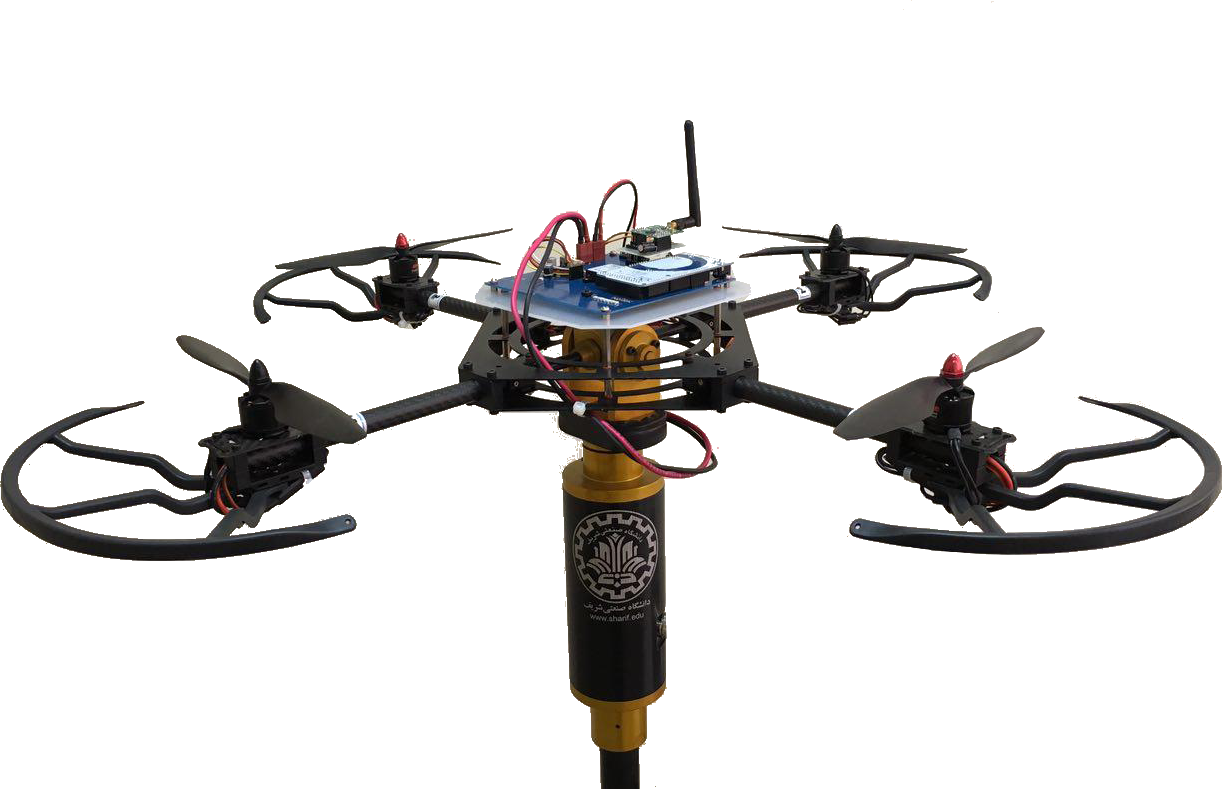
\includegraphics[width=0.7\textwidth]{../Figure/3DOFQuad.png}
    \caption{3DoF setup of the quadrotor.}
    \label{fig:quadrotor}
 \end{figure}
 
 \begin{figure}[H]
    \centering
    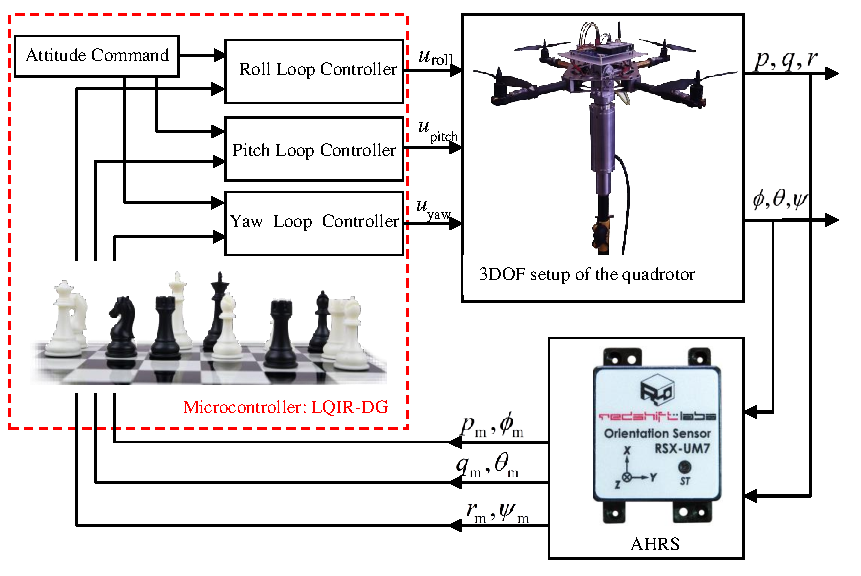
\includegraphics[width=0.7\textwidth]{../Figure/schematic.pdf}
    \caption{Structure of the LQIG-DG Controller Illustrated in a Block Diagram.}
    \label{fig:blockdiagram}
 \end{figure}
 \section{Dynamic Model of the Quadrotor Platform}\label{sec:modeling}
 \noindent In this section, first, a nonlinear model for the quadrotor platform is derived. Then, a state-space model and a linear model are developed for control purposes to be utilized in a controller strategy. Finally, a nonlinear identification method is applied to identify the parameters of the quadrotor.
 \subsection{Quadrotor Configuration}
\noindent Figure \ref{fig:schematic} shows the quadrotor schematic. It depicts four rotors rotating around the $z_B$ axis in the coordinate system of the body. The rotors have a rotational velocity of $\Omega_r$.
The quadrotor platform has 3 degrees of freedom, including roll, pitch, and yaw motions, which are described by roll $(\phi)$, pitch $(\theta)$, and yaw $(\psi)$ angles, respectively.
The counterclockwise rotation of Rotors 1 and 3 generates a moment that counteracts the yawing moment, while the clockwise rotation of Rotors 2 and 4 produces a moment that also counteracts the yawing moment.
\begin{figure}[H]
    \centering
    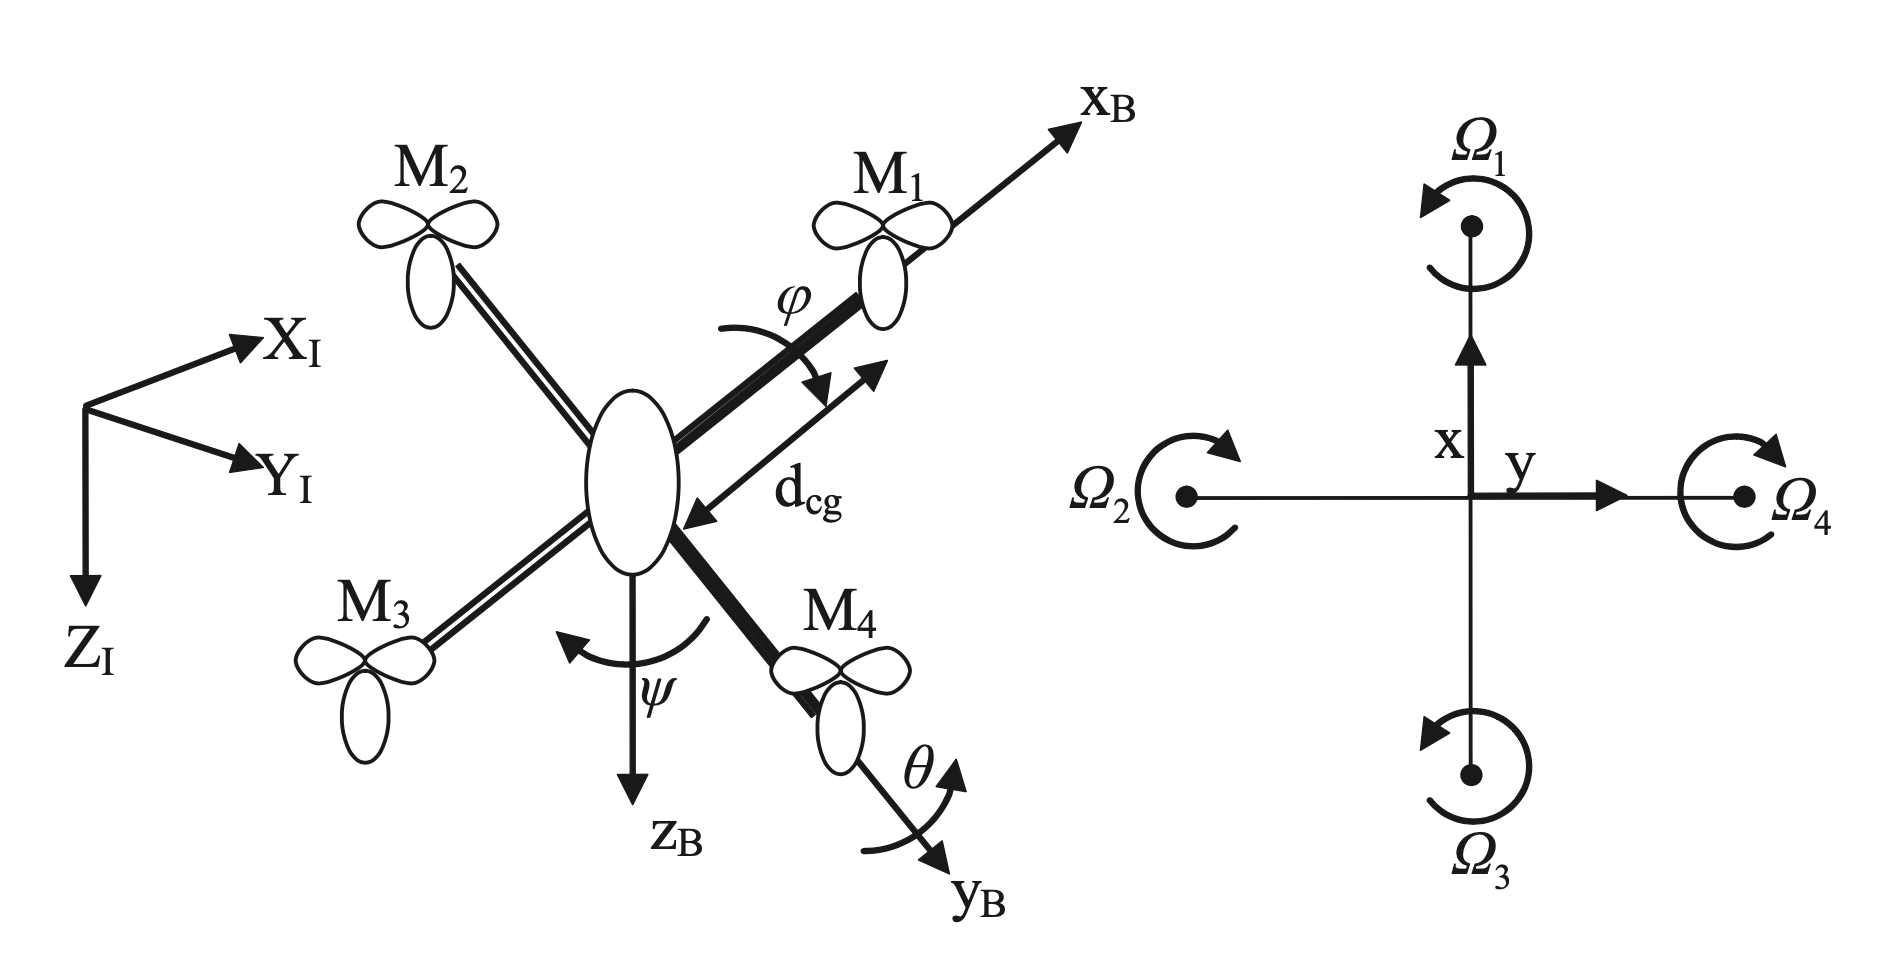
\includegraphics[width=12cm]{../Figure/schematic.png}
    \caption{Quadrotor Configuration.}
    \label{fig:schematic}
\end{figure}
\subsection{Dynamic Modeling of the Quadrotor Platfrorm}
\noindent Here, according to Newton-Euler, the dynamic model of the quadrotor platform is derived as follows \cite{4399042, article_Bouabdallah}:
\begin{align}
&\dot p = \dfrac{\mathrm{I}_{\text{yy}} - \mathrm{I}_{\text{zz}}}
{\mathrm{I}_{\text{xx}}} qr + q \dfrac{\mathrm{I}_{\text{rotor}}}
{\mathrm{I}_{\text{xx}}}\Omega_r + \dfrac{u_{\text{roll}}}{\mathrm{I}
_{\text{xx}}} + \dfrac{d_{\text{roll}}}{\mathrm{I}_{\text{xx}}}
\\
&\dot q = \dfrac{\mathrm{I}_{\text{zz}} - 
\mathrm{I}_{\text{xx}}}{\mathrm{I}_{\text{yy}}} rp +
p \dfrac{\mathrm{I}_{\text{rotor}}}{\mathrm{I}_{\text{xx}}}\Omega_r + 
\dfrac{u_{\text{pitch}}}{\mathrm{I}_{\text{yy}}} +
\dfrac{d_{\text{pitch}}}{\mathrm{I}_{\text{yy}}}
\\
&\dot r = \dfrac{\mathrm{I}_{\text{xx}} -
\mathrm{I}_{\text{yy}}}{\mathrm{I}_{\text{zz}}} pq 
+  \dfrac{u_{\text{yaw}}}{\mathrm{I}_{\text{zz}}} 
+ \dfrac{d_{\text{yaw}}}{\mathrm{I}_{\text{zz}}}
\end{align}
The $(p, q, r)$ represent the rotational variables, and $d_{\text{roll}}$, $d_{\text{pitch}}$, and $d_{\text{yaw}}$ denote the disturbances produced in the $x_B$, $y_B$, and $z_B$ axes, respectively. Additionally, $\mathrm{I}_{\text{xx}}$, $\mathrm{I}_{\text{yy}}$, and $\mathrm{I}_{\text{zz}}$ are the principal moments of inertia, and $\mathrm{I}_{\text{rotor}}$ is the rotor inertia about its axis. Euler angle rates are also determined from angular body rates as follows:
\begin{equation}
	\begin{bmatrix}
	\dot\phi \\
	\dot\theta \\
	\dot\psi
	\end{bmatrix}
	\begin{bmatrix}
	1 & \sin(\phi)\tan(\theta) & \cos(\phi)\tan(\theta) \\
	0 & \cos(\phi) & -\sin(\phi) \\
	0 & \sin(\phi)/\cos(\theta) & \cos(\phi)/\cos(\theta)
	\end{bmatrix}
	\begin{bmatrix}
	p \\
	q \\
	r
	\end{bmatrix}
\end{equation}
The residual rotor velocity, denoted by $\Omega_r$, is calculated as follows:
\begin{equation}
	\Omega_r = -\Omega_1 + \Omega_2 - \Omega_3 + \Omega_4
\end{equation}
\subsection{Input of the Dynamic Model}
\noindent The control inputs $u_{\text{roll}}$, $u_{\text{pitch}}$, and $u_{\text{yaw}}$ are to the moments generated by the quadrotor's rotors along the roll, pitch, and yaw axes, respectively, defined as follows:
\begin{align}
		&u_{\text{roll}} = \mathrm{b\,d}_{\text{cg}} (\Omega_2^2 - \Omega_4^2)\\
	&u_{\text{pitch}} = \mathrm{b\,d}_{\text{cg}} (\Omega_1^2 - \Omega_3^2) \\
	&u_{\text{yaw}} = \mathrm{d} (\Omega_1^2 - \Omega_2^2 + \Omega_3^2 - \Omega_4^2)
\end{align}
where $\mathrm{d}_{\text{cg}}$, $\text{d}$, and $\text{b}$ represent the distance between the rotors and the gravity center, drag factor, and thrust factor, respectively. The rotational velocity commands are computed as follows:
\begin{align}
    \Omega_{c, 1}^2 &= \Omega_{\text{mean}}^2 + \dfrac{1}{2\mathrm{b\,d}_{\text{cg}}}u_{\text{pitch}} + \dfrac{1}{4d}u_{\text{yaw}} \\
    \Omega_{c, 2}^2 &= \Omega_{\text{mean}}^2 + \dfrac{1}{2\mathrm{b\,d}_{\text{cg}}}u_{\text{roll}} - \dfrac{1}{4d}u_{\text{yaw}}\\
    \Omega_{c, 3}^2 &= \Omega_{\text{mean}}^2 - \dfrac{1}{2\mathrm{b\,d}_{\text{cg}}}u_{\text{pitch}} + \dfrac{1}{4d}u_{\text{yaw}} \\
    \Omega_{c, 4}^2 &= \Omega_{\text{mean}}^2 - \dfrac{1}{2\mathrm{b\,d}_{\text{cg}}}u_{\text{roll}} - \dfrac{1}{4d}u_{\text{yaw}}
\end{align}
In the above equation, $\Omega_{\text{mean}}$ is nominal rotational velocities of the rotors.

\subsection{State-Space Formulation}\label{sec:state-space}
\noindent Here, by defining $x_1 = p$, $x_2 = q$, $x_3 = r$, $x_4 = \phi$, $x_5 = \theta$, and $x_6 = \psi$, the formulation of the quadrotor platform is presented as follows:
\begin{align}\label{eq:diffeq}
	\dot x_1 &= \Gamma_1x_2 x_3 + \Gamma_2 x_2 \Omega_r + \Gamma_3u_{\text{roll}} + \Gamma_3d_{\text{roll}} \\[0.5em]
    \dot x_2 &= \Gamma_4 x_1 x_3 - \Gamma_5 x_1 \Omega_r +  \Gamma_6u_{\text{pitch}} + \Gamma_6d_{\text{pitch}}\\[0.5em] \label{eq:diffeq-mid}
    \dot x_3 &= \Gamma_7x_1 x_2 +  \Gamma_8u_{\text{yaw}} + \Gamma_8d_{\text{yaw}}\\[0.5em] 
    \dot x_4 &= x_1 + (x_2\sin(x_4) + x_3\cos(x_4))\tan(x_5)
    \\[0.5em]
    \dot x_5 &= x_2\cos(x_4) - x_3\sin(x_4)\\[0.5em]
    \dot x_6 &= (x_2\sin(x_4) + x_3\cos(x_4))/\cos(x_5) \label{eq:diffeq-end}
\end{align}
where $\Gamma_i (i = 1, \ldots, 8)$ is defined as:
\begin{equation}
	\begin{split}
		\Gamma_1 &= \dfrac{\mathrm{I}_{\text{yy}} - \mathrm{I}_{\text{zz}}}{\mathrm{I}_{\text{xx}}}, \quad \Gamma_2 = \dfrac{\mathrm{I}_{\text{rotor}}}{\mathrm{I}_{\text{xx}}}, \quad \Gamma_3 = \dfrac{1}{\mathrm{I}_{\text{xx}}}\\ \Gamma_4 &= \dfrac{\mathrm{I}_{\text{zz}} - \mathrm{I}_{\text{xx}}}{\mathrm{I}_{\text{yy}}}, \quad \Gamma_5 = \dfrac{\mathrm{I}_{\text{rotor}}}{\mathrm{I}_{\text{xx}}}, \quad \Gamma_6 = \dfrac{1}{\mathrm{I}_{\text{yy}}} \\ \Gamma_7 &= \dfrac{\mathrm{I}_{\text{xx}} - \mathrm{I}_{\text{yy}}}{\mathrm{I}_{\text{zz}}}, \quad \Gamma_8 = \dfrac{1}{\mathrm{I}_{\text{zz}}}
	\end{split}
\end{equation}
Moreover, the measurement vector, obtained from the AHRS sensor is presented as follows:
\begin{equation}
    \begin{split}
        \boldsymbol{\mathrm{z}} &= \begin{bmatrix}
        p \
        q \
        r \
        \phi \
        \theta \
        \psi
    \end{bmatrix}^\mathrm{T} + \boldsymbol{\nu}
    \end{split}
\end{equation}
where $\boldsymbol{\nu}$ is a Gaussian white noise. In the above equation, the superscripts $\mathrm{T}$ indicate the transpose notation.
\subsection{Linear Model}
\noindent The linear continuous-time model of the quadrotor platform about the equilibrium points $(\boldsymbol{{\mathrm{x}}}_e!=!0$ and $\boldsymbol{{\mathrm{u}}}_e!=!0)$ is represented as:
\begin{equation}\label{eq:linear}
	\boldsymbol{\dot{\mathrm{x}}}(t) = \boldsymbol{\mathrm{A\,x}}(t) + \boldsymbol{\mathrm{B\,u}}(t) + \boldsymbol{\mathrm{B_{d}\,d}}(t)
\end{equation}
where $\boldsymbol{\dot{\mathrm{x}}} = \begin{bmatrix}
				\boldsymbol{{\mathrm{\dot x_{\text{roll}}}}}&
				\boldsymbol{{\mathrm{\dot x_{\text{pitch}}}}}&
				\boldsymbol{{\mathrm{\dot x_{\text{yaw}}}}}
\end{bmatrix}$, defined as:
\begin{equation}
	\begin{split}
		\boldsymbol{\mathrm{x}}_{\text{roll}} = \begin{bmatrix}
			p \\ \phi
		\end{bmatrix}, \quad
		\boldsymbol{\mathrm{x}}_{\text{pitch}} = \begin{bmatrix}
			q \\ \theta \end{bmatrix} \quad
		\boldsymbol{\mathrm{x}}_{\text{yaw}} = 
		\begin{bmatrix}
			r \\ \psi
		\end{bmatrix}
	\end{split}
\end{equation}
Moreover, $\boldsymbol{\mathrm{B}}$ and $\boldsymbol{\mathrm{B_d}}$ are the input and disturbance matrices, respectively, and are defined as:
\begin{equation}
	\boldsymbol{\mathrm{B}} = \boldsymbol{\mathrm{B_d}} = 
	\begin{bmatrix}
		\boldsymbol{{\mathrm{B_{\text{roll}}}}} & \boldsymbol{0} & \boldsymbol{0}\\
		\boldsymbol{0} & \boldsymbol{{\mathrm{B_{\text{pitch}}}}} & \boldsymbol{0} \\
		\boldsymbol{0} & \boldsymbol{0} & \boldsymbol{{\mathrm{B_{\text{yaw}}}}}
	\end{bmatrix}
\end{equation}
In addition, the input matrices and state are shown as:
\begin{equation}
	\begin{split}
		\boldsymbol{\mathrm{A}}_{\text{roll}}  =\boldsymbol{\mathrm{A}}_{\text{pitch}}  = \boldsymbol{\mathrm{A}}_{\text{yaw}}  = \begin{bmatrix}
			0 & 0\\
			1 & 0
		\end{bmatrix}
	\end{split}
\end{equation}
\begin{equation}
	\begin{split}
		\boldsymbol{\mathrm{B}}_{\text{roll}}  = \begin{bmatrix}
			\dfrac{1}{\mathrm{I}_{\text{xx}}}
			\\[1em]
			0
		\end{bmatrix};~ \boldsymbol{\mathrm{B}}_{\text{pitch}}  = \begin{bmatrix}
			\dfrac{1}{\mathrm{I}_{\text{yy}}}
			\\[1em]
			0
		\end{bmatrix};~ \boldsymbol{\mathrm{B}}_{\text{yaw}}  = \begin{bmatrix}
			\dfrac{1}{\mathrm{I}_{\text{zz}}}
			\\[1em]
			0
		\end{bmatrix}
	\end{split}
\end{equation}
\subsection{Identification of the Platform Parameters}
\noindent This section describes the utilization of the Nonlinear Least Squares (NLS) algorithm for estimating the model parameters ($\boldsymbol{\mathrm{\Gamma}}$) of the 3DoF experimental platform using experimental data.
This technique is based on the Trust-Region Reflective Least Squares (TRRLS) method, which iteratively finds the values of the model parameters by minimizing a cost function, defined as follows:
\begin{equation}
	\min_{\Gamma_i}\left(\parallel e(\Gamma_i) \parallel^2\right) = 
	\min_{\Gamma_i} = \left(\sum_{j=1}^{n}(\boldsymbol{z}_j- \hat{\boldsymbol{z}}_j)(\boldsymbol{z}_j- \hat{\boldsymbol{z}}_j)^\mathrm{T}\right)
\end{equation}

\begin{figure}[H]
	\centering
    \resizebox{1\textwidth}{!}{
	\begin{tikzpicture}[font=\small,thick]
		% Start block
		\node[draw, align=center,		minimum width=2.5cm,		minimum height=1cm, fill=blue!10] (block1) {\textbf{Experimental Data} \\Input: rotational velocity\\
		Output: attitude};
			
		% Voltage and Current Measurement
		\node[draw, align=center,		below=of block1,		minimum width=3.5cm,		minimum height=1cm, fill=blue!10	] (block2) {\textbf{Data Preprocessing} \\ Synchronization experimental, vs simulated data.};
		
		% Power and voltage variation
		
		\node[draw, align=center,		below=of block2,		minimum width=3.5cm,		minimum height=1cm, fill=blue!10	] (block3) {\textbf{NLS-TRRLS Optimization}\\
		Set bounds for parameters\\
		Set initial seed for all parameters\\
		Minimization of the cost function.};

		\node[draw, align=center,	below right=of block3,	minimum width=3cm,	minimum height=2.5cm,	fill=green!10	] (block_p) {{Identified parameters}\\
		$\boldsymbol\Gamma = \begin{bmatrix}\Gamma_1 &
			\Gamma_2 & \Gamma_3 & \Gamma_4\\
			\Gamma_5 & \Gamma_6 & \Gamma_7 & \Gamma_8
		\end{bmatrix}$};

		\node[draw, align=center,	below left=of block3,	minimum width=3cm,	minimum height=2.5cm,	fill=red!10	] (block_s) {{simulated model}\\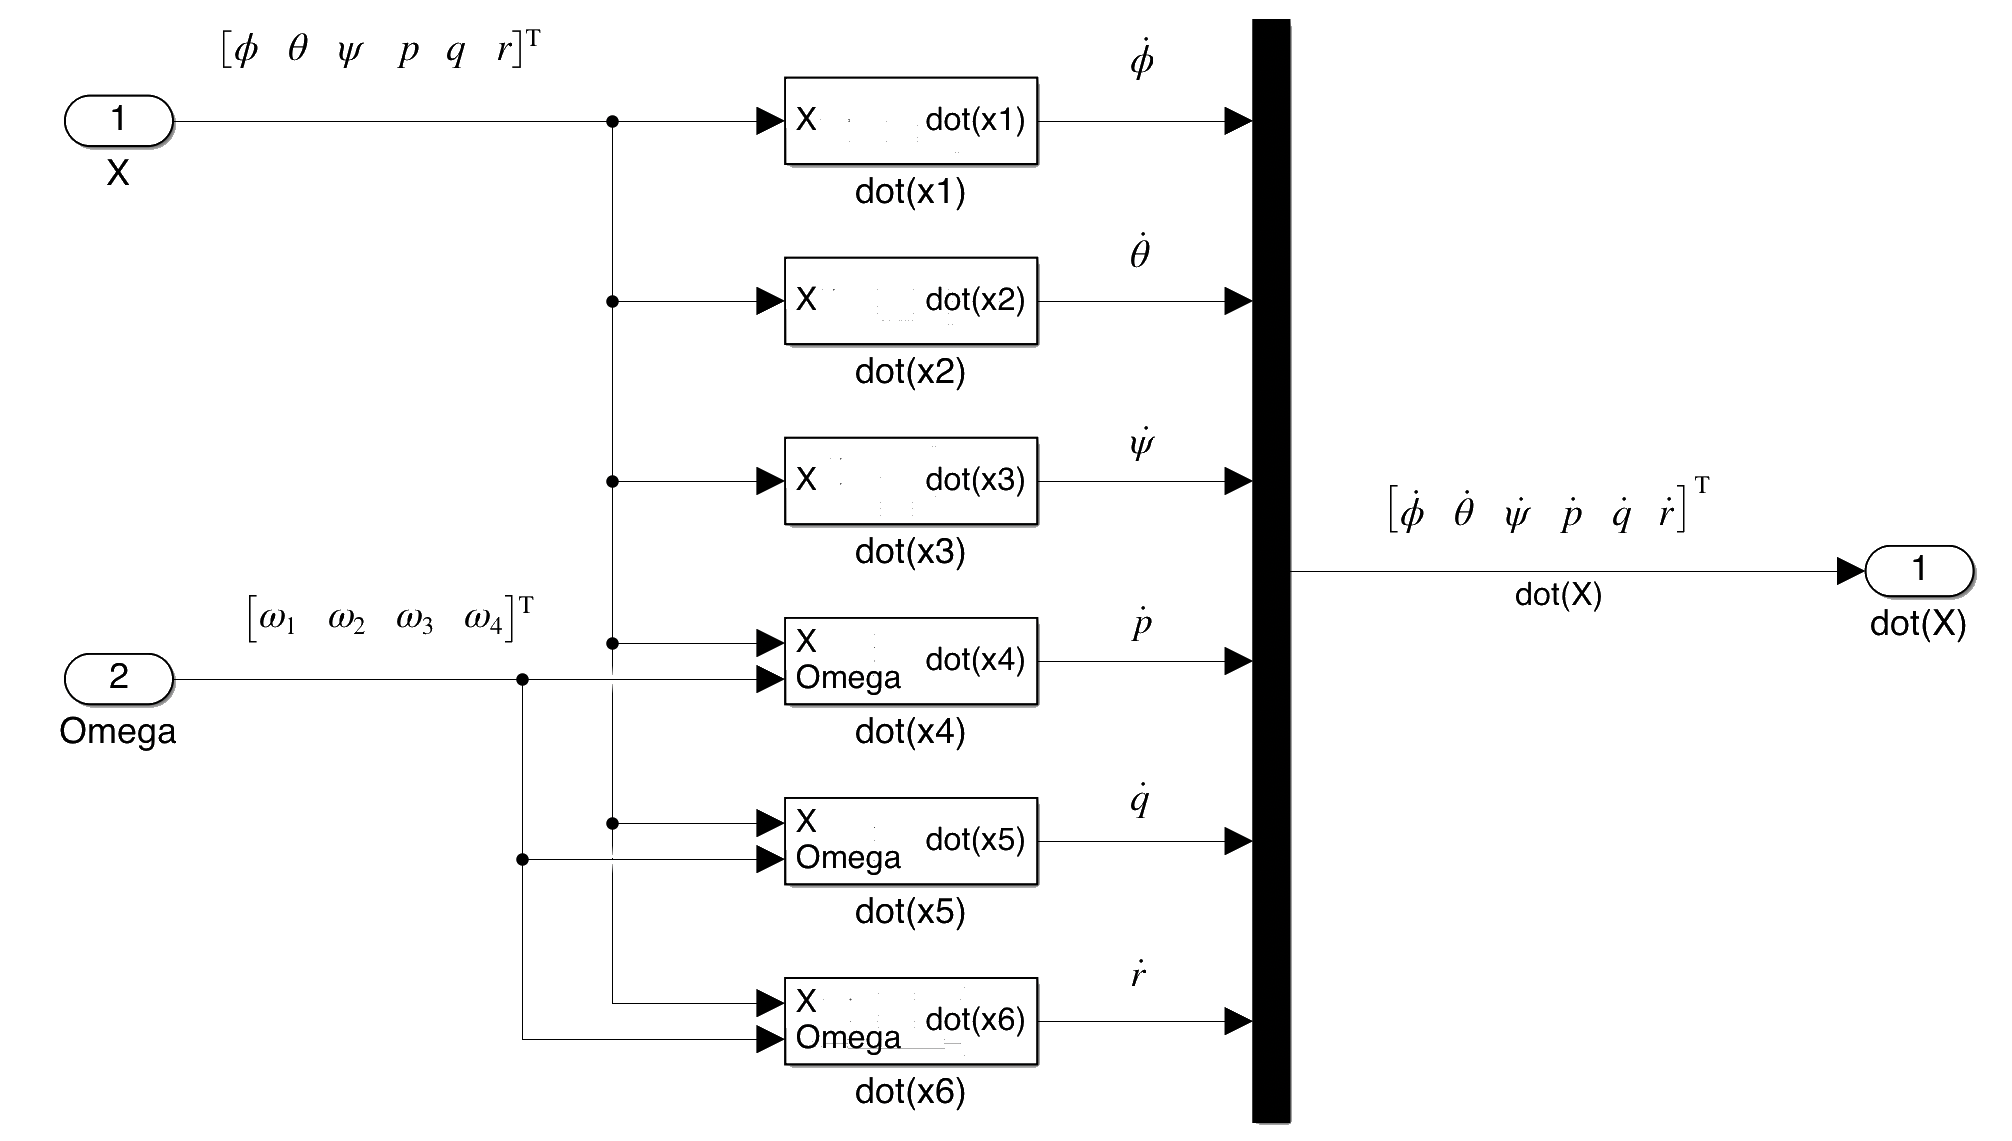
\includegraphics[scale=.05]{../Figure/All-six.png}};
		
		% Conditions test
		\node[draw,		diamond,		below =4cm of block3,		minimum width=2.5cm,		inner sep=0,		fill=yellow!10	] (block4) { Error $< \delta$};
		
		\node[draw,		below=1.5cm of block4,		minimum height=1cm,		minimum width=2.5cm,		inner sep=0,		fill=blue!10	] (block5) {End};
		
		\node[draw,		right=2cm of block4,		minimum height=1cm,		minimum width=2.5cm,		fill=red!10		] (block6) {Insufficient experimental data};
				
		 
		 
		% Arrows
		\draw[-latex] (block1) edge (block2)
			(block2) edge (block3)
			(block3) -| (block_s);
			% (block3) edge (block_p);
	
		\draw[-latex] (block3) -| (block_p);
	
		\draw[-latex] (block_s) -| (block4);
	
		\draw[-latex] (block_p) -| (block4);
	
		\draw[stealth-stealth] (block_s) -- (block_p);
		 
		\draw[-latex] (block4) -- (block5)
			node[pos=0.5,fill=white,inner sep=0]{Yes};
		 
		\draw[-latex] (block4) -- (block6)
			node[pos=0.5,fill=white,inner sep=0]{No};
	
		\coordinate[left=5.5cm of block3] (aux);
		\coordinate[right= of block_p] (aux1);
		% \draw[-latex] (block6) |- (block2);
		\draw[-latex] (block1) -| (aux) |- (block4);
		\draw[-latex] (block6) -| (aux1) |- (block1);
		\end{tikzpicture}
        }
		\caption{Structure of TRRLS identification approach.}
		\label{fig:identification}
\end{figure}
\section{Formulation of the LQDG Controller}\label{sec:controller}
\noindent Here, the LQR-DG controller is augmented with an integral action to eliminate steady-state errors. For this purpose, the augmented states of the quadrotor platform, which include states and their integrals, are selected. The design methodology of the LQR-DG controller is introduced. It generates optimal control signals for the three degrees of freedom platform.
\subsection{Augmented State Space Development}
\noindent To integrate the integrator into the control strategy architecture, the augmented state variables are defined below:
\begin{equation}\label{lqidg_x}
    \boldsymbol{\mathrm{x_{a_i}}} = \begin{bmatrix}
        \boldsymbol{\mathrm{x_i}} \\[1em]
        \displaystyle\int\boldsymbol{\mathrm{x_i}}
    \end{bmatrix}
\end{equation}
The dynamics model of the quadrotor, as expressed by Eq. \eqref{eq:linear}, is reformulated into an augmented state-space model that incorporates the roll ($\phi$), pitch ($\theta$), and yaw ($\psi$) angles. The augmented state-space model provides a comprehensive description of the quadrotor's dynamic behavior, enabling the design of effective control strategies. The ensuing state-space model that integrates the augmented state variables is mathematically represented and defined in the following manner:
\begin{equation}\label{systemlqidg}
	\begin{split}
		\boldsymbol{\dot{\mathrm{x}}_a}(t) &= \boldsymbol{\mathrm{A_ax_a}}(t) + \boldsymbol{\mathrm{B_{{a}}u}}(t) + \boldsymbol{\mathrm{B_{{d_a}}d}}(t)%, \quad \boldsymbol{x}(0) = 
	\end{split}
\end{equation}
$\boldsymbol{\mathrm{B_a}}$ and $\boldsymbol{\mathrm{A_a}}$, which are expressed as below:
\begin{equation}
	\boldsymbol{\mathrm{B_a}} = \boldsymbol{\mathrm{B_{{d_a}}}} = \begin{bmatrix}
		\boldsymbol{\mathrm{B}}\\
		\boldsymbol{0}
	\end{bmatrix}
\end{equation}

\begin{equation}
	\boldsymbol{\mathrm{A_a}} = \begin{bmatrix}
		\boldsymbol{\mathrm{A}} & \boldsymbol{0}\\
		\boldsymbol{\mathrm{I}} & \boldsymbol{0}
	\end{bmatrix}
\end{equation}
In the aforementioned expression, the notation $\boldsymbol{\mathrm{I}}$ denotes the identity matrix.
\subsection{LQR-DG Control Scheme with Integral Action}
\noindent In line with the principles of differential game theory, the LQIR-DG controller is designed to be both robust and optimal.
The LQIR-DG scheme involves selecting two fundamental players, one responsible for determining the control command and the other for generating the worst possible disturbance. To achieve the primary objective, the primary player minimizes the following cost function, while the other player must maximize it:
\begin{equation}
    \min_{u} \max_{d} J(\boldsymbol{\mathrm{x_{a_i}}}, {d_i}, {u_i}) = J(\boldsymbol{\mathrm{x_{a_i}}}, {u^*_i}, {d^*_i})=\min_{d} \max_{u}
     \int_{0}^{\mathrm{t_f}}\biggl (\boldsymbol{\mathrm{x^\mathrm{T}_{a_i}}}  \boldsymbol{\mathrm{Q_i}} \boldsymbol{\mathrm{x_{a_i}}}+
    {{u^\mathrm{T}_i}}  {{R}} {{u_i}}-
    {{d^\mathrm{T}_{i}}} {{ R_{d} d_{i}}}
    \biggl )\mathrm{d}t
\end{equation}
where $\boldsymbol{\mathrm{Q_i}}$, ${{R_{d}}}$, and ${{R}}$ are weight coefficients of the function. The final time is denoted by $\mathrm{t_f}$.
By solving the above problem, the control command is computed as follows \cite{LQDG}:
\begin{equation}
	{{d_i}}(t) =\boldsymbol{{\mathrm{K_{d_i}}}}(t)\boldsymbol{{\mathrm{x_{a_i}}}}(t)
\end{equation}
Moreover, the worst disturbance is obtained as:
\begin{equation}
		{{u_i}}(t) = -\boldsymbol{{\mathrm{K}}_{i}}(t) \boldsymbol{{\mathrm{x_{a_i}}}}(t)
\end{equation}
Here, $\boldsymbol{{\mathrm{K_{d_i}}}}$ and $\boldsymbol{{\mathrm{K_i}}}$ are gain values defined as follows:
\begin{align}
	\boldsymbol{{\mathrm{K_i}}} &= {{{R}}^{-1}}\boldsymbol{{\mathrm{B}_{a_i}^\mathrm{T}}}\boldsymbol{{\mathrm{P}}_{a_i}}(t)\\
	\boldsymbol{{\mathrm{K_{d_i}}}} &= {{{R}}^{-1}_{d}}\boldsymbol{{\mathrm{B}_{a_{d_i}}^\mathrm{T}}}\boldsymbol{{\mathrm{P}}_{a_{d_i}}}(t)
\end{align}
where $\boldsymbol{{\mathrm{P}}_{a_i}}(t)$ and $\boldsymbol{{\mathrm{P}}_{a_{d_i}}}(t)$ satisfy
\begin{align}\label{coupled_riccatti_LQIDG}
	&-\boldsymbol{\mathrm{A^\mathrm{T}_a}}\boldsymbol{\mathrm{P_{a_{d_i}}}}(t)
	 - \boldsymbol{\mathrm{Q_{i}}} - \boldsymbol{\mathrm{P_{a_{d_i}}}}(t)\boldsymbol{\mathrm{A_a}} 
	 + \boldsymbol{\mathrm{P_{a_{d_i}}}}(t)\boldsymbol{\mathrm{S_{a_i}}}(t)\boldsymbol{\mathrm{P_{a_i}}}(t)
	  +\boldsymbol{\mathrm{P_{a_{d_i}}}}(t)\boldsymbol{\mathrm{S_{a_{d_i}}}}(t)\boldsymbol{\mathrm{P_{a_{d_i}}}}(t)
	=\boldsymbol{\mathrm{0}}\\
            &-\boldsymbol{\mathrm{A^\mathrm{T}_a}}\boldsymbol{\mathrm{P_{a_i}}}(t) - \boldsymbol{\mathrm{Q_i}}
			 - \boldsymbol{\mathrm{P_{a_i}}}(t)\boldsymbol{\mathrm{A_a}}  +
			  \boldsymbol{\mathrm{P_{a_i}}}(t)\boldsymbol{\mathrm{S_{a_{d_i}}}}(t)\boldsymbol{\mathrm{P_{a_{d_i}}}}(t) 
			  +\boldsymbol{\mathrm{P_{a_i}}}(t)\boldsymbol{\mathrm{S_{a_i}}}(t)\boldsymbol{\mathrm{P_{a_i}}}(t) =\boldsymbol{\mathrm{0}}
\end{align}
where $$
	\boldsymbol{\mathrm{S_{a_i}}} = \boldsymbol{\mathrm{B_{a_i}}}R^{-1}\boldsymbol{\mathrm{B}^\mathrm{T}_{a_i}}, \quad
	\boldsymbol{\mathrm{S{a_{d_i}}}} = \boldsymbol{\mathrm{B}_{a_{d_i}}}R_{d}^{-1}\boldsymbol{\mathrm{B}^\mathrm{T}_{a_{d_i}}}
$$
\section{Result and Discussion}\label{sec:results}
\noindent Here, the simulation results of parameter identification and LQIDG-Controller for a quadrotor platform are presented. First, the quadrotor parameters are estimated based on the NLS method. Then, the performance of the LQDG controller structure is evaluated. The performance of the quadrotor LQIDG controller is presented in Tables \ref{tab:parameters} and \ref{tab:control weight_new}.
\begin{table}[H]
	\renewcommand{\arraystretch}{1.3}
	\caption{Quadrotor Parameters}
	\begin{center}
	\begin{tabular}{c c c}
	\hline
	\textbf{Parameter} & \textbf{\textit{Value}}& \textbf{\textit{Unit}} \\
	\hline
	$\mathrm{d}_{\text{cg}}$  & $0.2$ & $\mathrm{m}$\\
	$\mathrm{d}$  & $3.2\times10^{-6}$ & $\mathrm{N.m.\sec^2/rad^2}$\\
	$\mathrm{b}$  & $3.13\times10^{-5}$ & $\mathrm{N.\sec^2/rad^2}$ \\
	$\mathrm{I}_{\text{xx}}$ & $0.02839$ & $\mathrm{kg.m^2}$ \\
	$\mathrm{I}_{\text{yy}}$  & $0.03066$ & $\mathrm{kg.m^2}$\\
	$\mathrm{I}_{\text{zz}}$  & $0.0439$ & $\mathrm{kg.m^2}$ \\
	$\mathrm{I}_{\text{rotor}}$  & $4.4398\times 10^{-5}$ & $\mathrm{kg.m^2}$\\
	
	
	$\Omega_{\text{mean}}$ & $3000$ & $\mathrm{rpm}$\\
	
	\hline
	\end{tabular}
	\label{tab:parameters}
	\end{center}
\end{table}
\begin{table}[H]
	\centering
	\caption{LQIR-DG Controller Parameters}
	\renewcommand{\arraystretch}{1.3}
	\begin{tabular}{@{}lll@{}}
	\toprule
	\textbf{Channel} & \textbf{Weighting Matrix} & \textbf{Matrix Values} \\
	\midrule
	Roll & $\mathbf{Q_{roll}}$ & $\text{diag}([0.02, 65.96, 83.04, 0.00])$ \\
	Pitch & $\mathbf{Q_{pitch}}$ & $\text{diag}([435.01, 262.60, 262.60, 0.00])$ \\
	Yaw & $\mathbf{Q_{yaw}}$ & $\text{diag}([4 \times 10^{-4}, 0.00, 0.133, 0])$ \\
	& $\mathbf{R}$ & $1$ \\
	&$\mathbf{R_d}$ & $1.2764$ \\
	\bottomrule
	\end{tabular}
	\label{tab:control weight_new}
\end{table}
\subsection{Identification of the 3DoF quadrotor platform model}
\noindent As described in section \ref{sec:state-space}, the parameters of the quadrotor platform, denoted by $\Gamma_i (i=1, ..., 8)$, are identified using the NRS algorithm. The NLS-TRRLS algorithm is implemented in Matlab R2022b\textregistered.
To increase the accuracy of parameter identification, three scenarios according to Table \ref{tab:identification}.
In the first scenario, depicted in Figure \ref{fig:one_degree_identification}, the quadrotor is rotated about only one axis (roll, pitch, or yaw axes) to identify the parameters $\Gamma_3$, $\Gamma_6$, and $\Gamma_8$.
In the second scenario, as illustrated in Figure \ref{fig:two_degree_identification}, the parameters $\Gamma_2$ and $\Gamma_5$ are estimated by moving the experimental platform to freely rotate around its roll and pitch axes simultaneously. 
When the stopping condition of the NLS algorithm is met, the optimal values of the quadrotor parameters are computed and presented in Table \ref{tab:true_parameters}. 
These results illustrate that the outputs of the simulation results for the quadrotor model are consistent with reality.
\begin{table}[H]
	\caption{Scenarios for Identification of Quadrotor Parameters.}
	\centering
	\begin{adjustbox}{max width=\textwidth}
	\begin{tabular}{*{9}{c}}
	\toprule
	\multirow{2}{*}{\textbf{Scenario}} & \multirow{2}{*}{\textbf{\textit{Description}}}
	& \multicolumn{3}{c}{\textbf{\textit{Initial Condition (deg)}}} &
	\multicolumn{4}{c}{\textbf{\textit{Rotational Velocity Commands}}} \\
	\cmidrule(lr){3-5} \cmidrule(lr){6-9}
	& & $\phi$ & $\theta$ & $\psi$ & $\Omega_1$ & $\Omega_2$ & $\Omega_3$ & $\Omega_4$\\
	\midrule
	\multirow{3}{*}{I} & Roll free & 38 & - & - & 2000 & 2000 & 2000 & 3400\\
	& Pitch free & - & -15 & - & 3700 & 2000 & 2000 & 2000 \\
	& Yaw free & -& - &-75 & 2000 & 3300 & 2000 & 3300 \\
	\midrule
	II & Roll and Pitch free &8 & -5 & - & 1700 & 3800 & 2400 & 1700\\
	\midrule
	III & Roll, Pitch, and Yaw free &
	8 & -3 & -146 & 1700 & 3800 & 2400 & 1700 \\
	\bottomrule
	\end{tabular}
	\end{adjustbox}
	\label{tab:identification}
\end{table}
\begin{table}[H]
	\renewcommand{\arraystretch}{1.3}
	\caption{True values of the quadrotor parameters.}
	\begin{center}
	\begin{tabular}{c c c c}
	\hline
	\textbf{Parameter} & \textbf{\textit{Value}}& \textbf{Parameter} & \textbf{\textit{Value}}  \\
	\hline
	$\Gamma_1$ & $-0.9622$ & $\Gamma_5$ & $3.6441\times10^{-4}$ \\

	$\Gamma_2$ & $-0.0154$ & $\Gamma_6$ & $7.5395\times10^{-5}$ \\

	$\Gamma_3$ &$5.4716\times10^{-5}$ & $\Gamma_7$ & $0.1308$ \\

	$\Gamma_4$ & $1.0457$ & $\Gamma_8$ & $4.3753\times10^{-5}$ \\
	\hline
	\end{tabular}
	\label{tab:true_parameters}
	\end{center}
\end{table}
\begin{figure}[H]
	\centering
	\subfloat[]{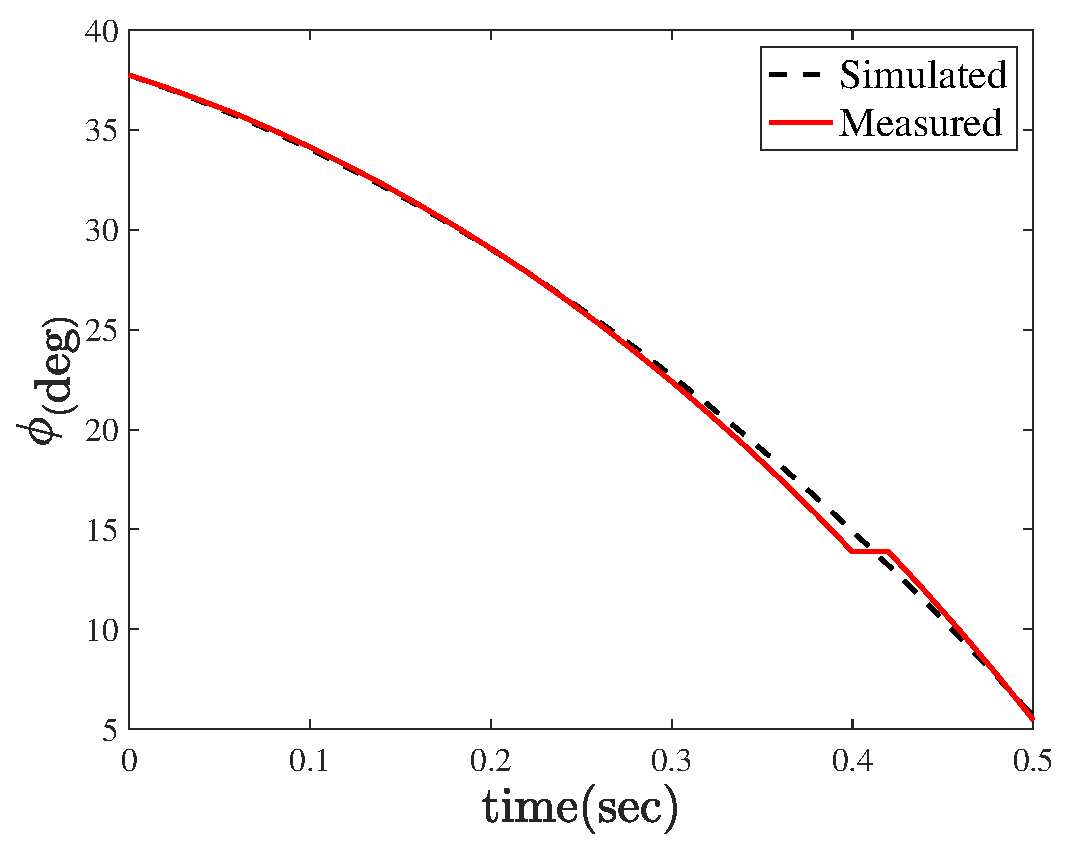
\includegraphics[width=.45\linewidth]{../Figure/parameter_estimation/roll/roll}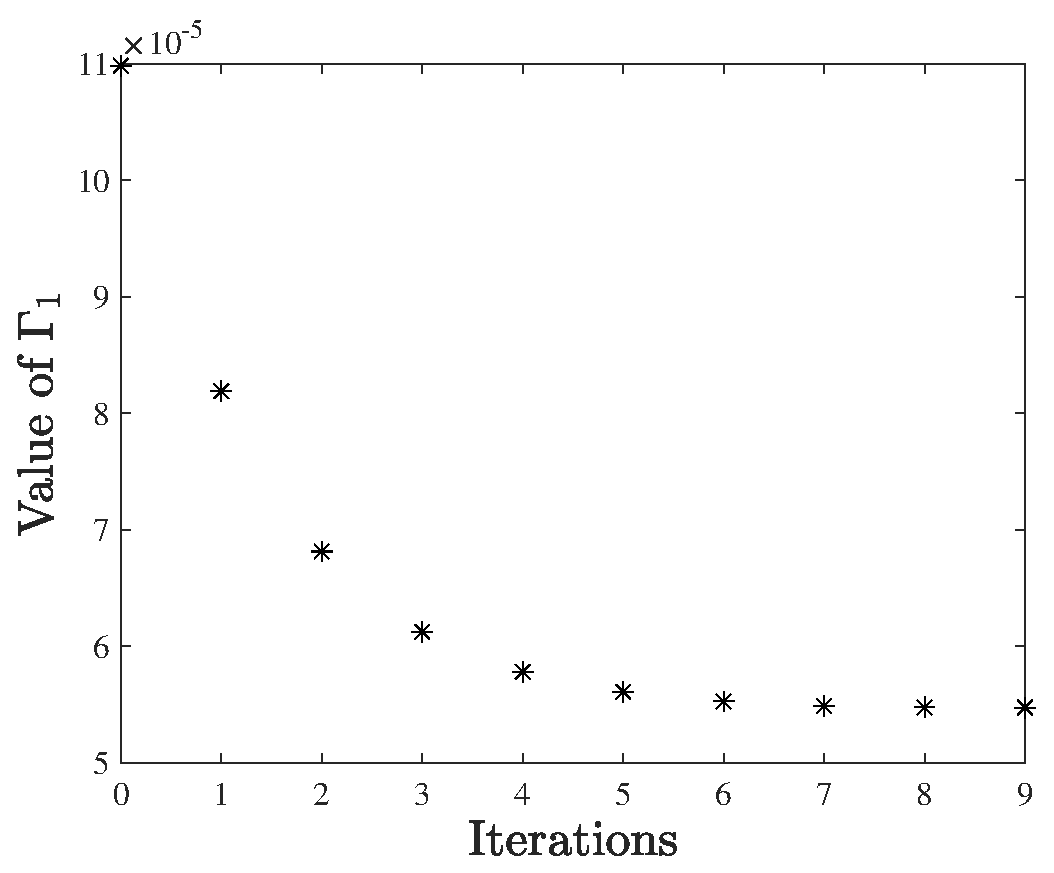
\includegraphics[width=.45\linewidth]{../Figure/parameter_estimation/roll/roll_parameter}
	}
	\hfil
	% \vspace{-0.25cm}
	\subfloat[]{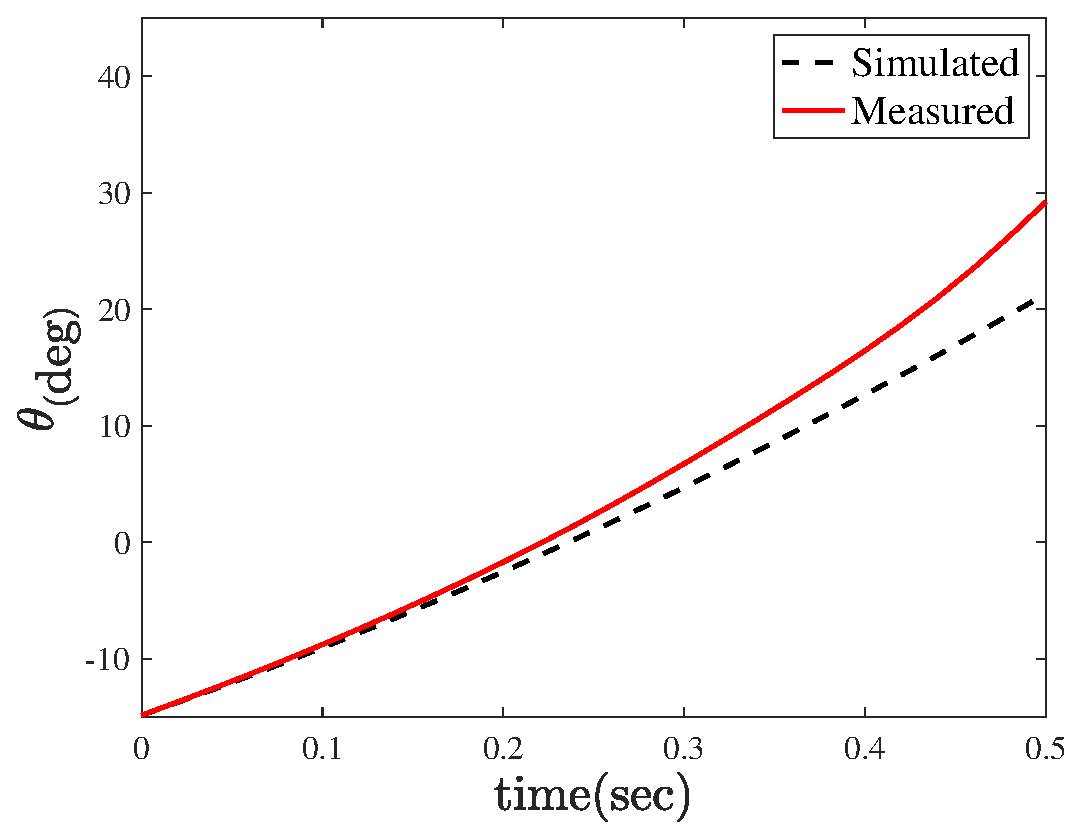
\includegraphics[width=.45\linewidth]{../Figure/parameter_estimation/pitch/pitch}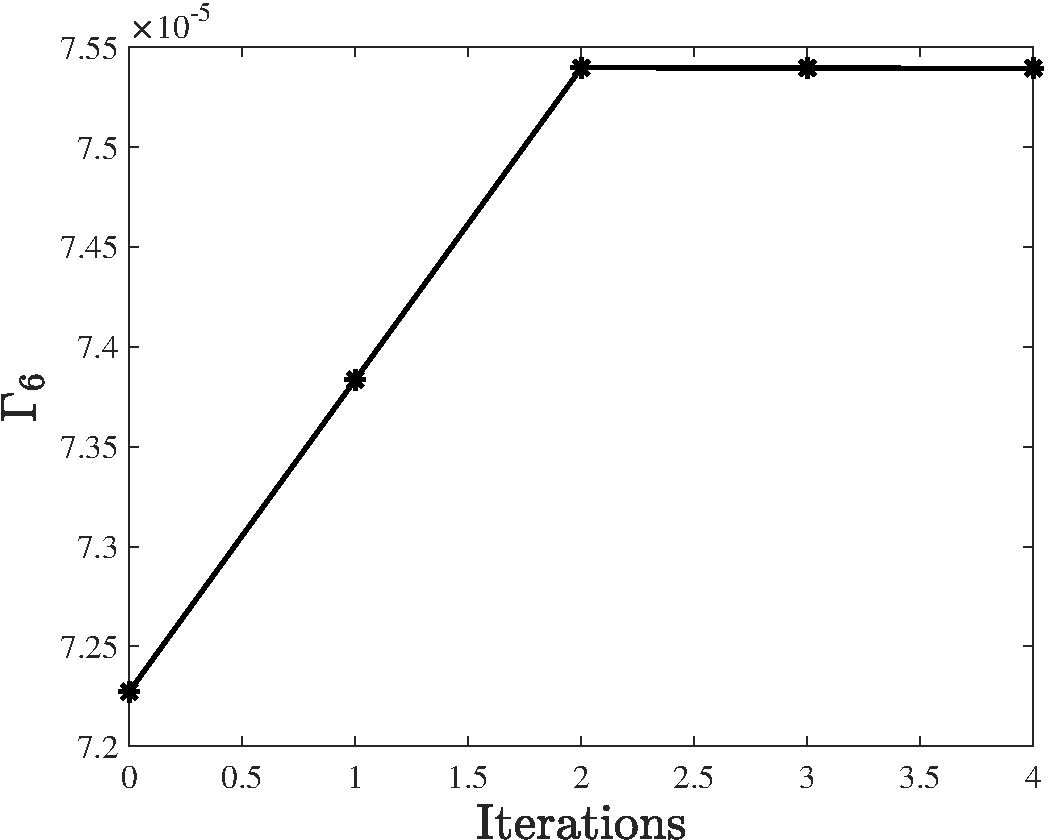
\includegraphics[width=.45\linewidth]{../Figure/parameter_estimation/pitch/pitch_parameter}
	}
	\hfil
	% \vspace{-0.25cm}
	\subfloat[]{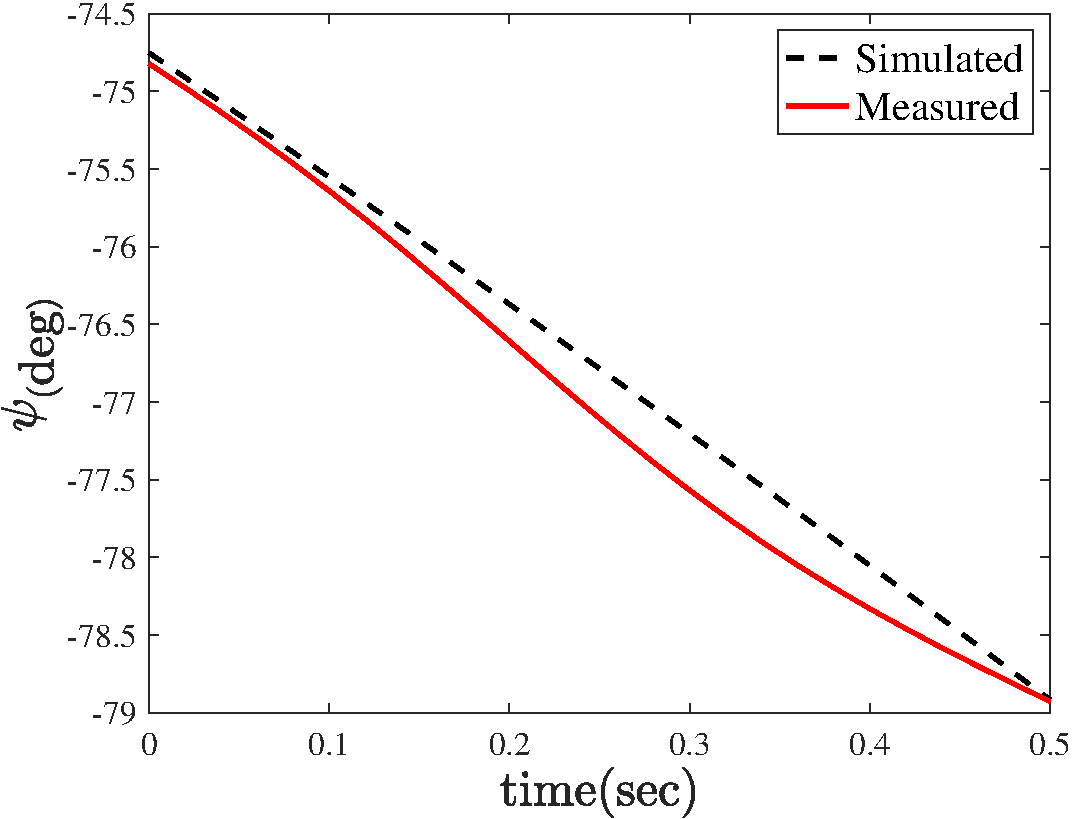
\includegraphics[width=.45\linewidth]{../Figure/parameter_estimation/yaw/yaw}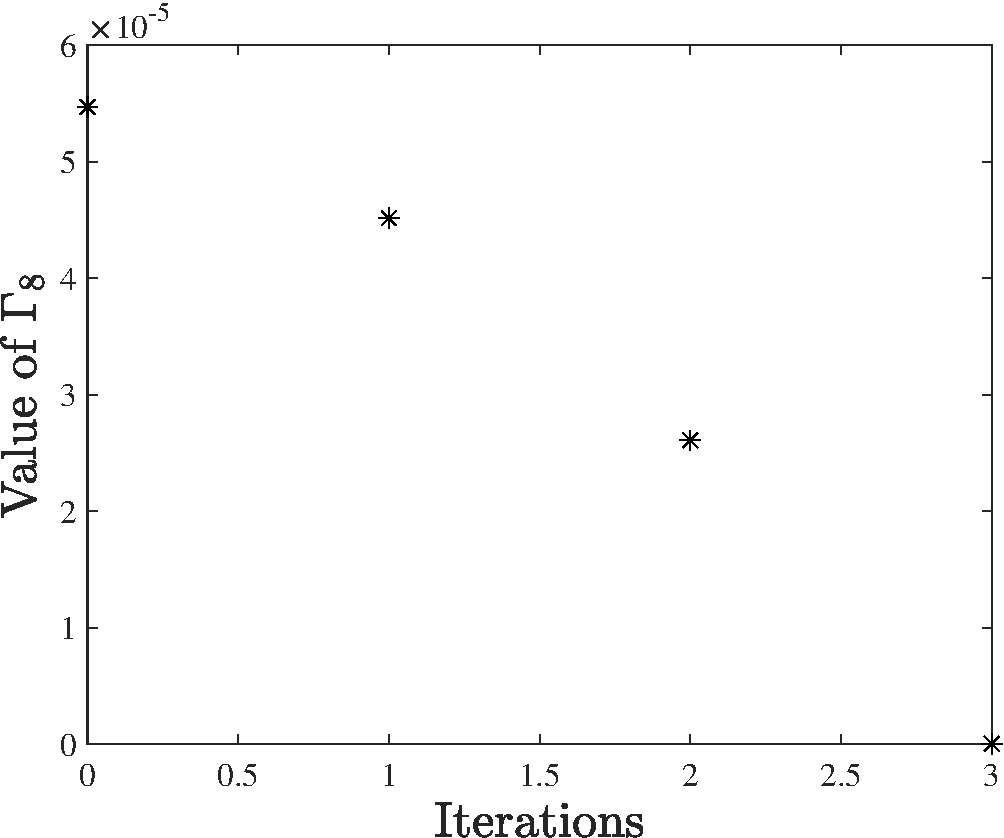
\includegraphics[width=.45\linewidth]{../Figure/parameter_estimation/yaw/yaw_parameter}
	}
	\caption{Identification process results when the quadrotor rotates about only one axis: (a) Identification of $\Gamma_3$ in free roll motion. (b) Identification of $\Gamma_6$ in free pitch motion. (c) Identification of $\Gamma_8$
	in free yaw motion.}
	\label{fig:one_degree_identification}
\end{figure}
\begin{figure}[H]
	\centering
	\subfloat[]{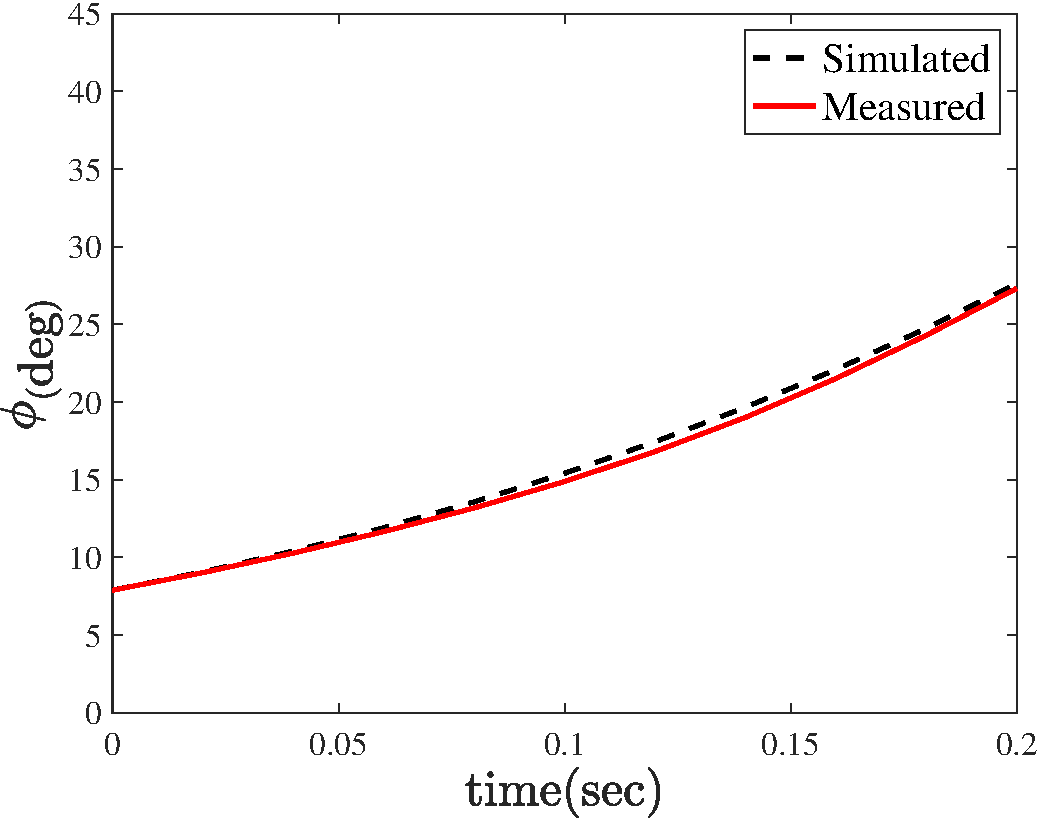
\includegraphics[width=.45\linewidth]{../Figure/parameter_estimation/roll-pitch/roll}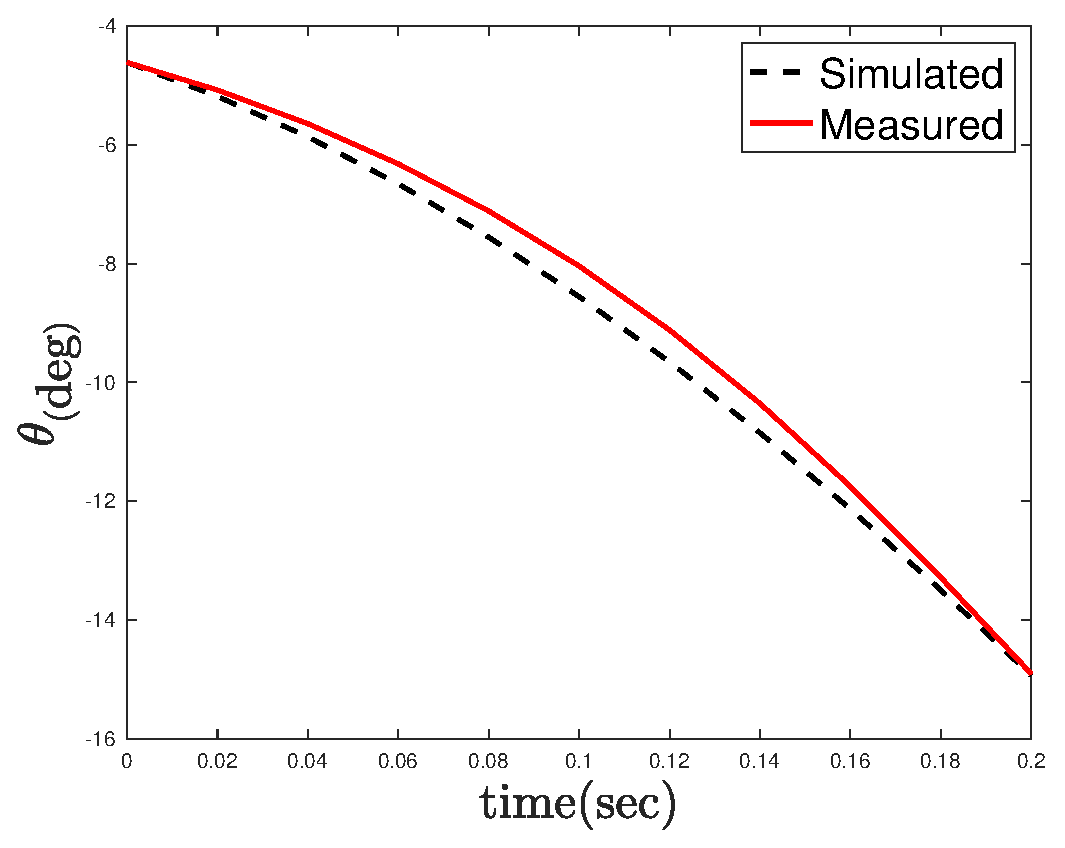
\includegraphics[width=.45\linewidth]{../Figure/parameter_estimation/roll-pitch/pitch}
	}
	\hfil
	% \vspace{-0.25cm}
	\subfloat[]{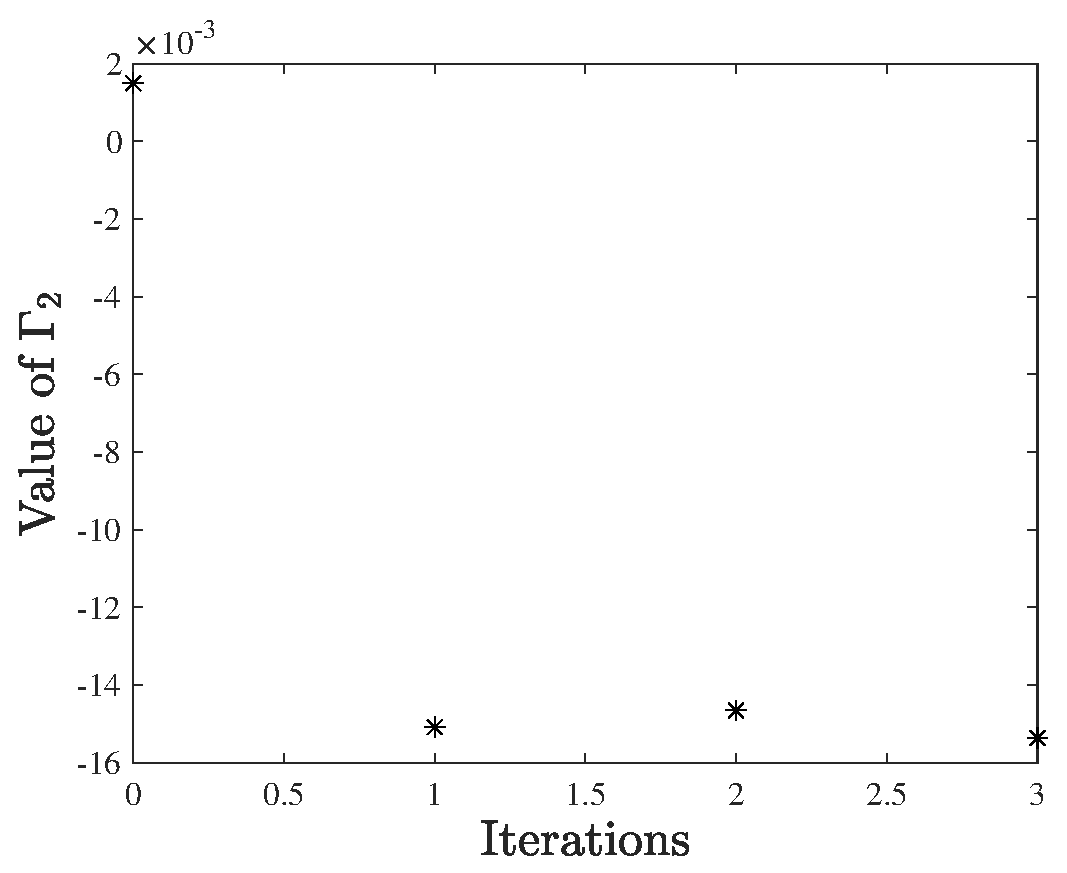
\includegraphics[width=.45\linewidth]{../Figure/parameter_estimation/roll-pitch/roll_parameter}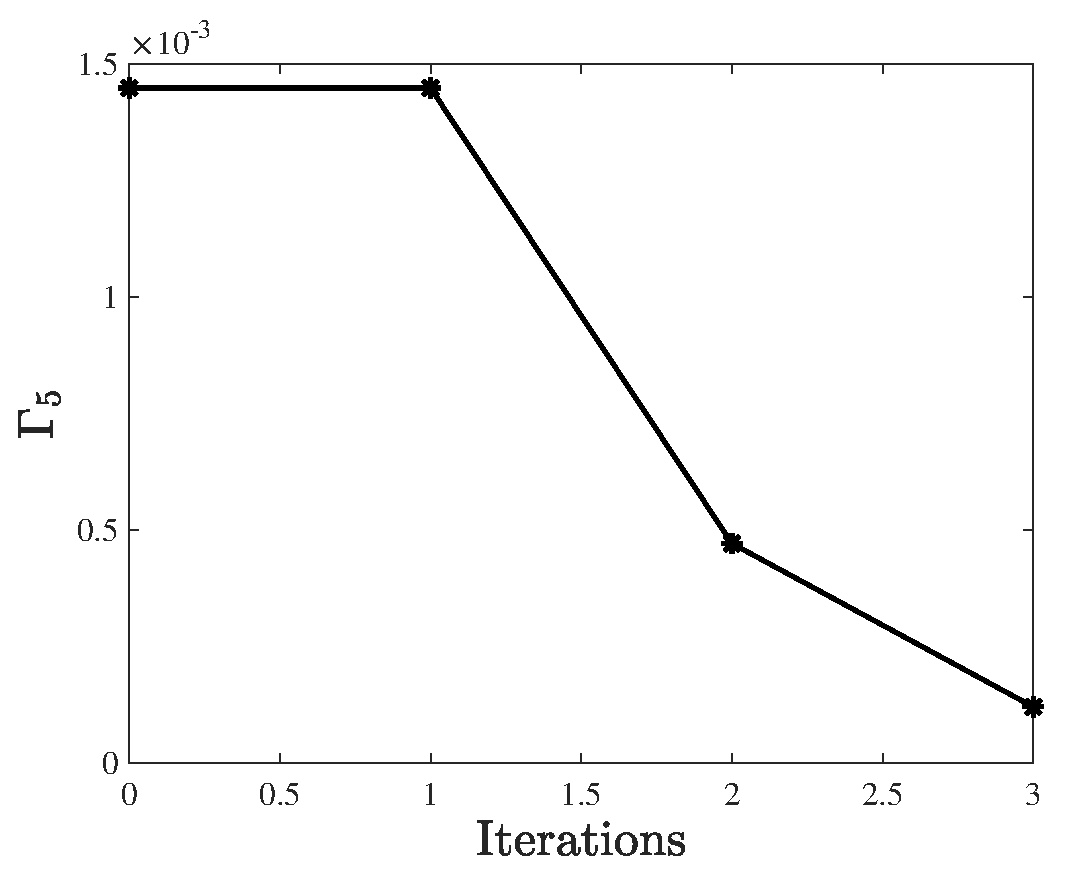
\includegraphics[width=.45\linewidth]{../Figure/parameter_estimation/roll-pitch/pitch_parameter}
	}
	\caption{Identification process results when the quadrotor rotates about its roll and pitch axes:
	(a) Comparison of Simulation and experimental results. (b) Identification of $\Gamma_2$ and $\Gamma_5$.}
	\label{fig:two_degree_identification}
\end{figure}
\begin{figure}[H]
	\centering
	\subfloat[]{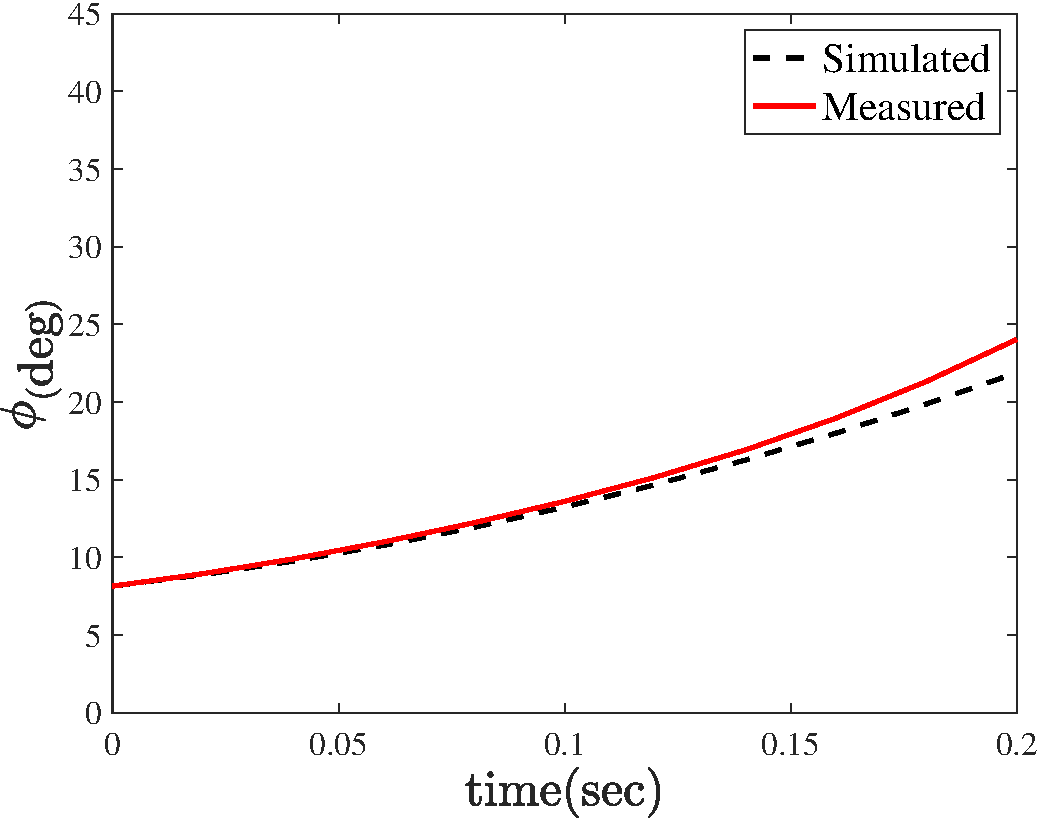
\includegraphics[width=.33\linewidth]{../Figure/parameter_estimation/3DOF/roll}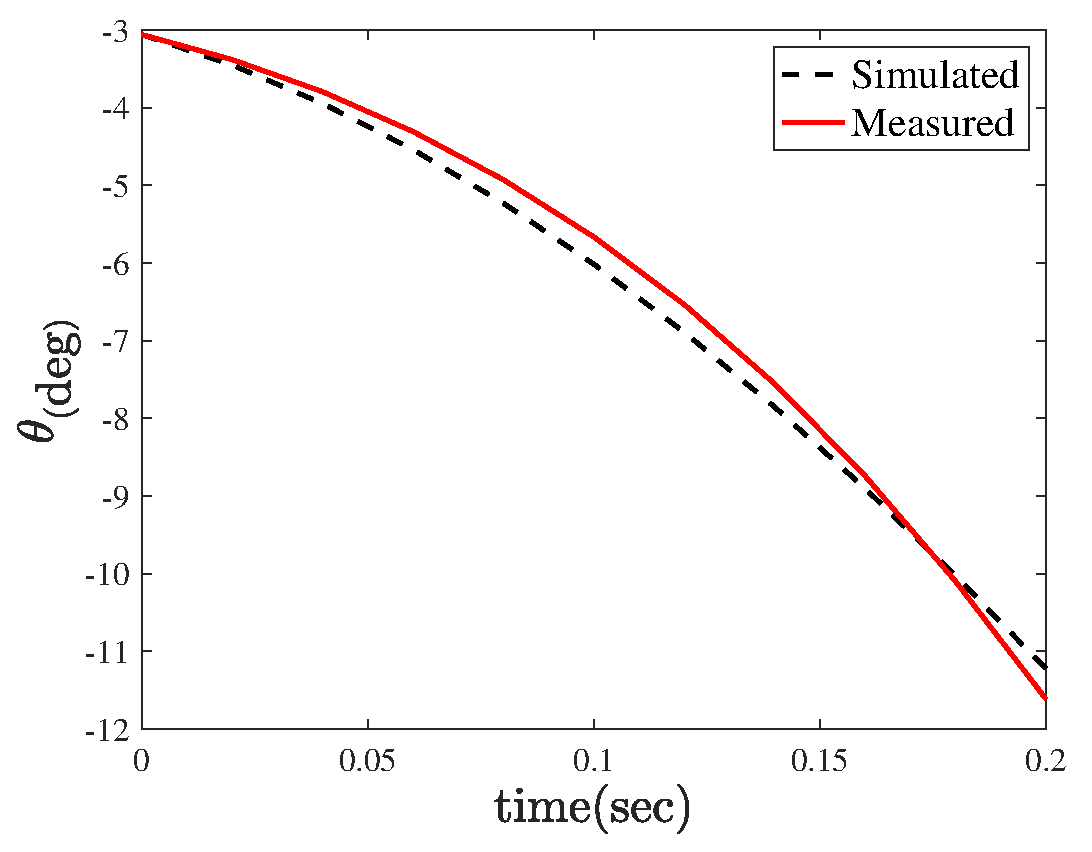
\includegraphics[width=.33\linewidth]{../Figure/parameter_estimation/3DOF/pitch}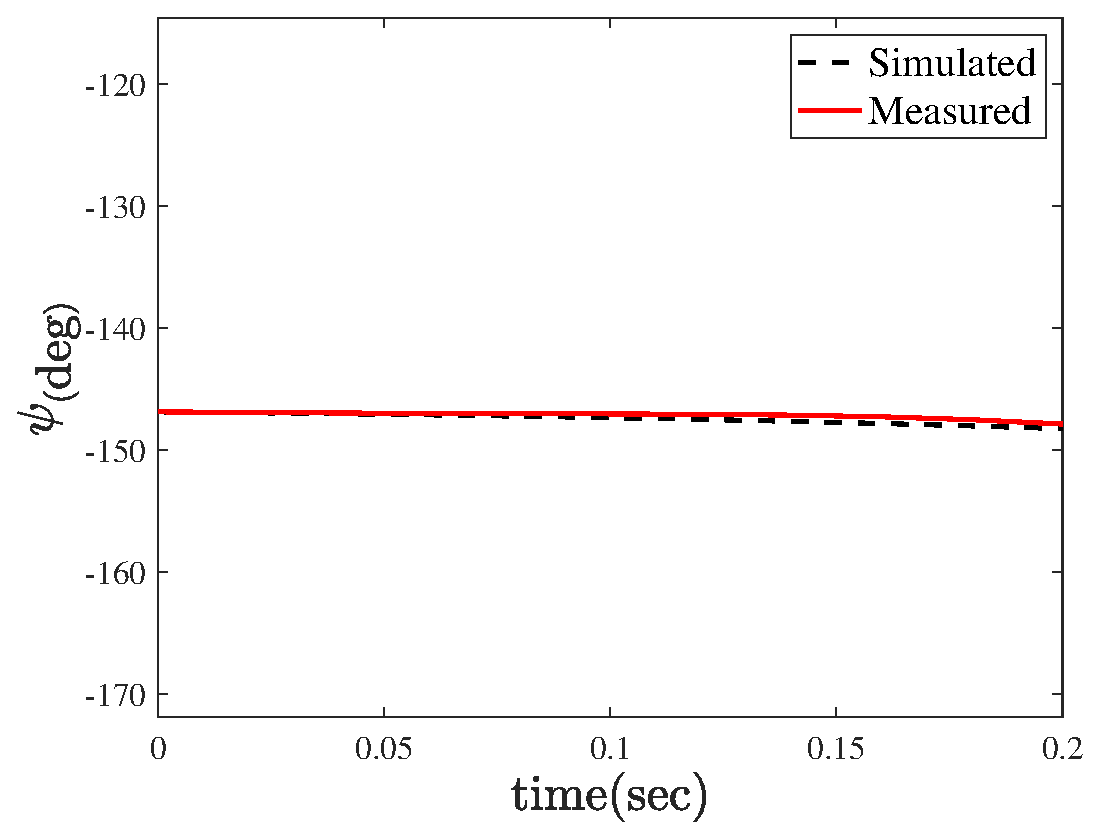
\includegraphics[width=.33\linewidth]{../Figure/parameter_estimation/3DOF/yaw}
	}
	\hfil
	\subfloat[]{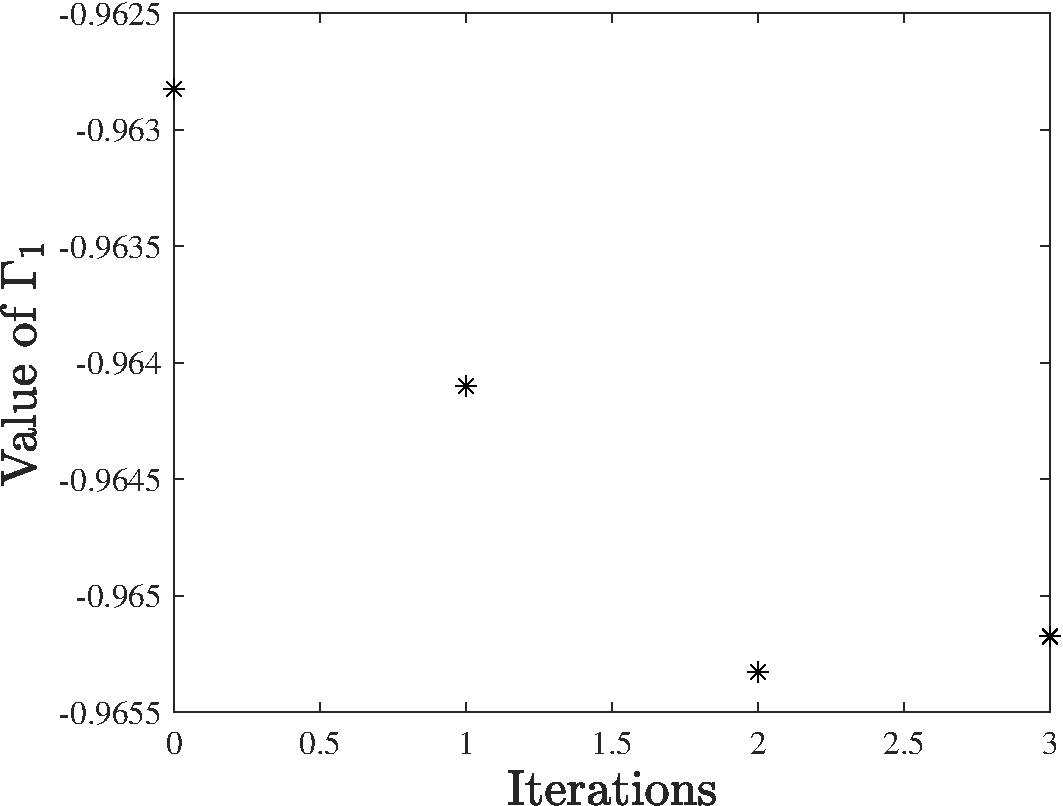
\includegraphics[width=.33\linewidth]{../Figure/parameter_estimation/3DOF/roll_parameter}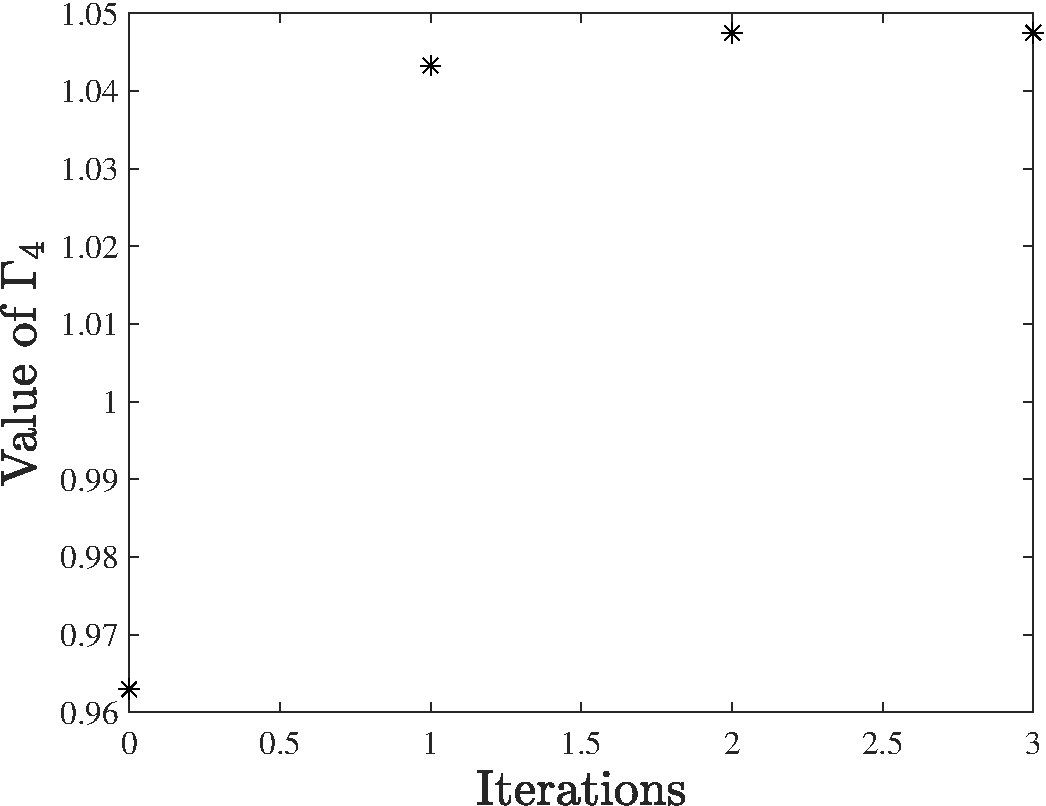
\includegraphics[width=.33\linewidth]{../Figure/parameter_estimation/3DOF/pitch_parameter}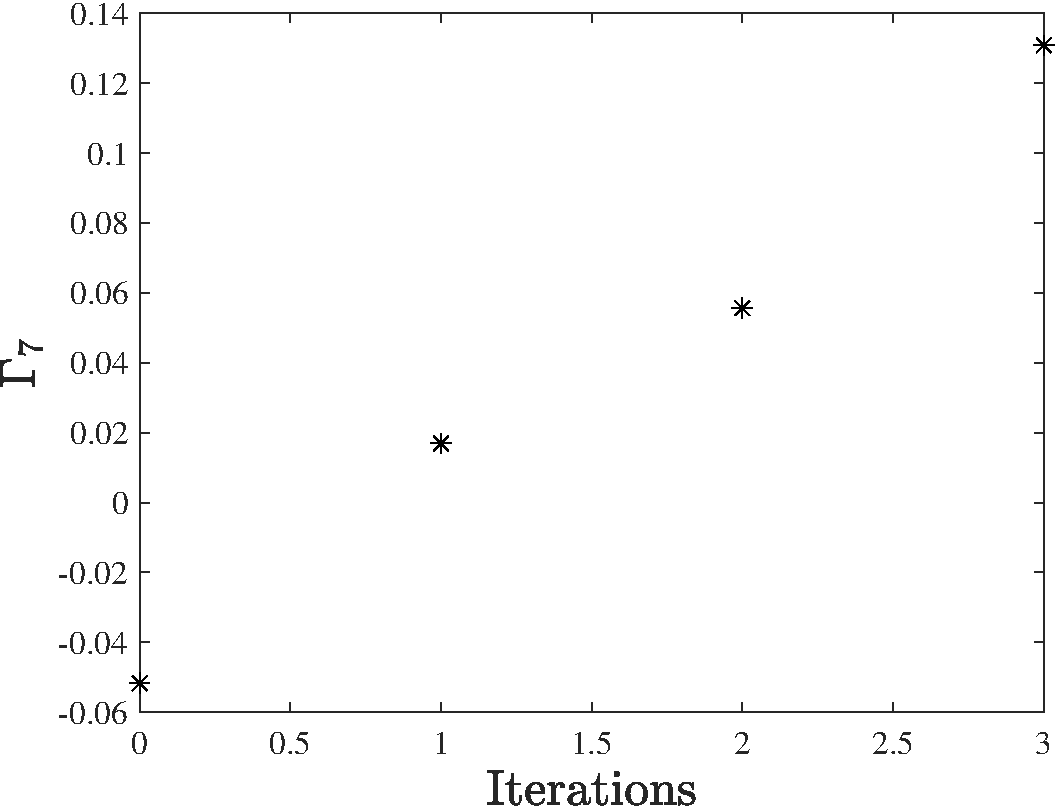
\includegraphics[width=.33\linewidth]{../Figure/parameter_estimation/3DOF/yaw_parameter}
	}
	\caption{Identification process results when the quadrotor rotates about its roll, pitch, and yaw axes: (a) Comparison of Simulation and experimental results. (b) Identification of $\Gamma_1$ , $\Gamma_4$ and
	$\Gamma_7$ parameters.}
	\label{fig:three_degree_identification}
\end{figure}
\subsection{Evaluation of LQIR-DG Performance}
\noindent Here, the performance of the LQIR-DG controller algorithm is evaluated for regulation and tracking performance, disturbance rejection, and the impact of model uncertainty.
Finally, the performance of the proposed controller is compared to the PID controller and variants of the LQR controller. 
The parameters of the PID controller are presented in Table \ref{tab:PID_parameters}.
\begin{table}[H]
	\renewcommand{\arraystretch}{1.3}
	\caption{Parameters of PID Controller}
	\begin{center}
		\begin{tabular}{cccc}
		\hline
		\textbf{Channel} & \textbf{$K_p$} & \textbf{$K_i$} & \textbf{$K_d$} \\
		\hline
		Roll & 2.0 & 0.5 & 1.0 \\
		Pitch & 1.5 & 0.4 & 0.8 \\
		Yaw & 3.0 & 0.6 & 1.2 \\
		\hline
		\end{tabular}
		\label{tab:PID_parameters}
	\end{center}
\end{table}
\subsubsection{Performance of the LQIR-DG Controller}\label{sec:regulation}
\noindent Here, the results of the LQIR-DG controller method are presented for the control loops of the Euler angles of the experimental platform in Figures \ref{fig:result} and \ref{fig:omega}.
The performance of the proposed controller is evaluated in Figure \ref{fig:result}.
Figure \ref{fig:result} \ref{sub@fig:regulation} compares the desired and output signals, i.e., the Euler angles during regulation. Figure \ref{fig:result} \ref{sub@fig:square} compares the desired square wave input with a frequency of 0.02 Hz and an amplitude of 20 degrees with the output signals in the two-degree-of-freedom coupling mode.
Moreover, Figures \ref{fig:omega} \ref{sub@fig:omega_regulation} and \ref{sub@fig:omega_square} show the rotational velocity command of the quadrotor in the regulation and tracking problems, respectively. These results demonstrate that the roll, pitch, and yaw angles are accurately controlled by the proposed approach.
\begin{figure}[H]
	\centering
	\subfloat[\label{fig:regulation}]{{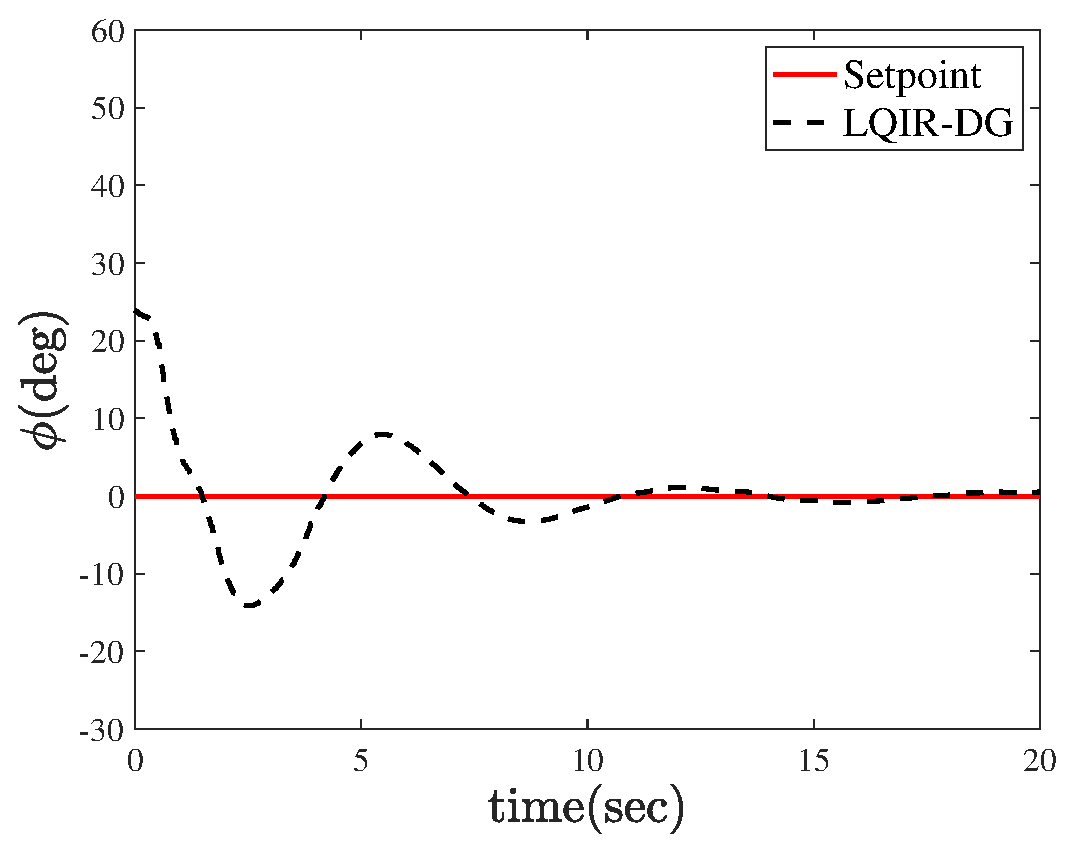
\includegraphics[width=.3\linewidth]{../Figure/implementation/lqidg_roll}}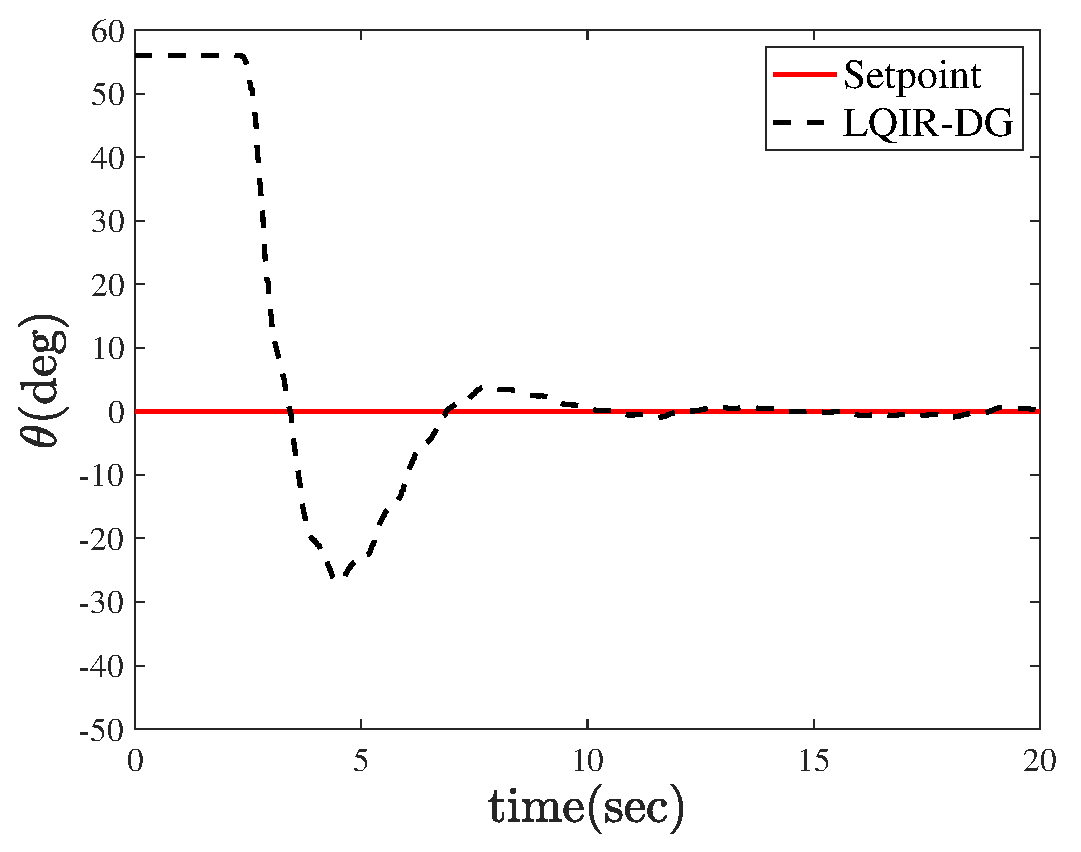
\includegraphics[width=.3\linewidth]{../Figure/implementation/lqidg_pitch}
	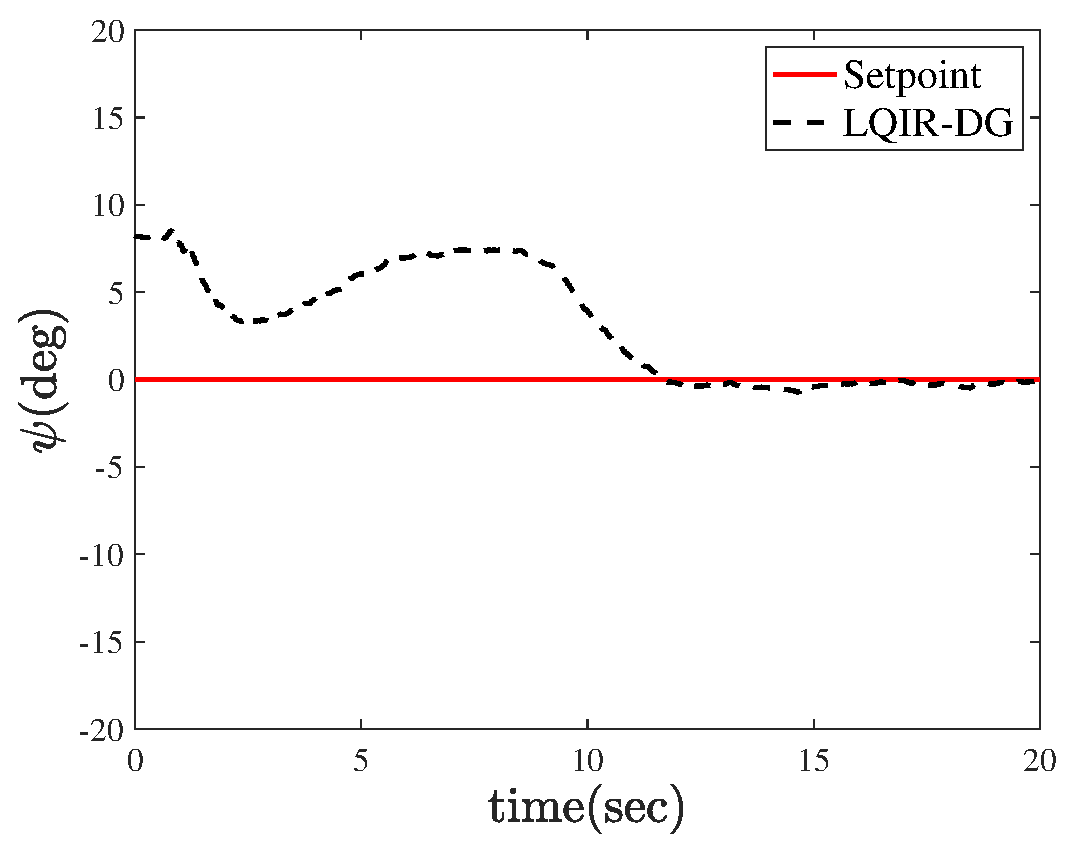
\includegraphics[width=.3\linewidth]{../Figure/implementation/lqidg_yaw}}
	\hfill
	\subfloat[\label{fig:square}]{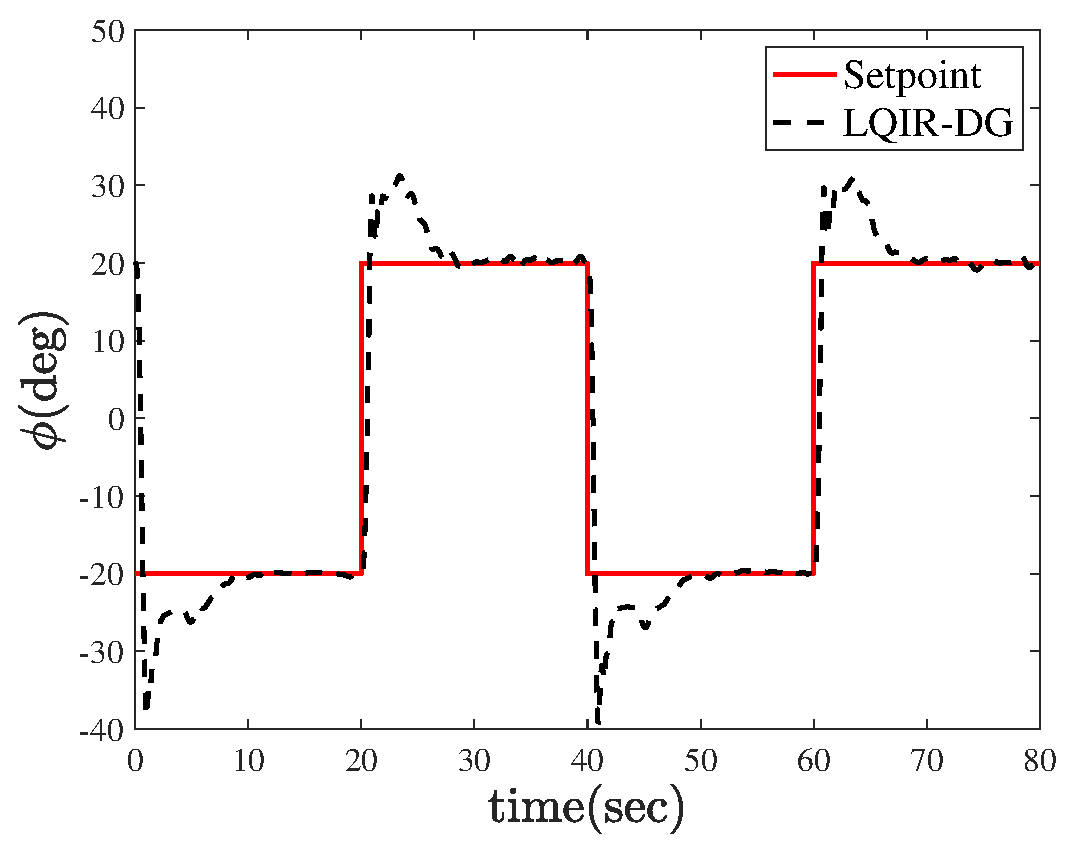
\includegraphics[width=.3\linewidth]{../Figure/implementation/square/lqidg_roll_20}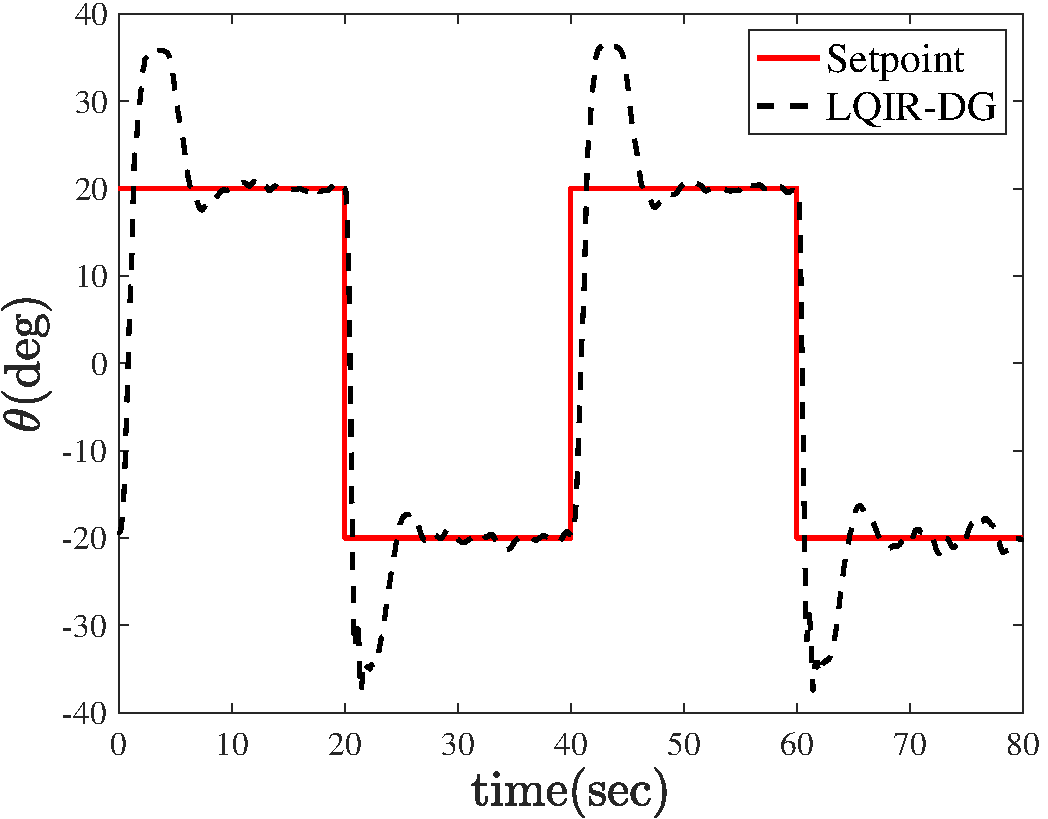
\includegraphics[width=.3\linewidth]{../Figure/implementation/square/lqidg_pitch_20}}
	\caption{Comparison of Euler angles in \ref{sub@fig:regulation} regulation \ref{sub@fig:square} Tracking Conditions}
	\label{fig:result}
\end{figure}

\begin{figure}[H]
	\centering
	\subfloat[\label{fig:omega_regulation}]{\includegraphics[width=.23\linewidth]{../Figure/implementation/lqidg_Omega_1}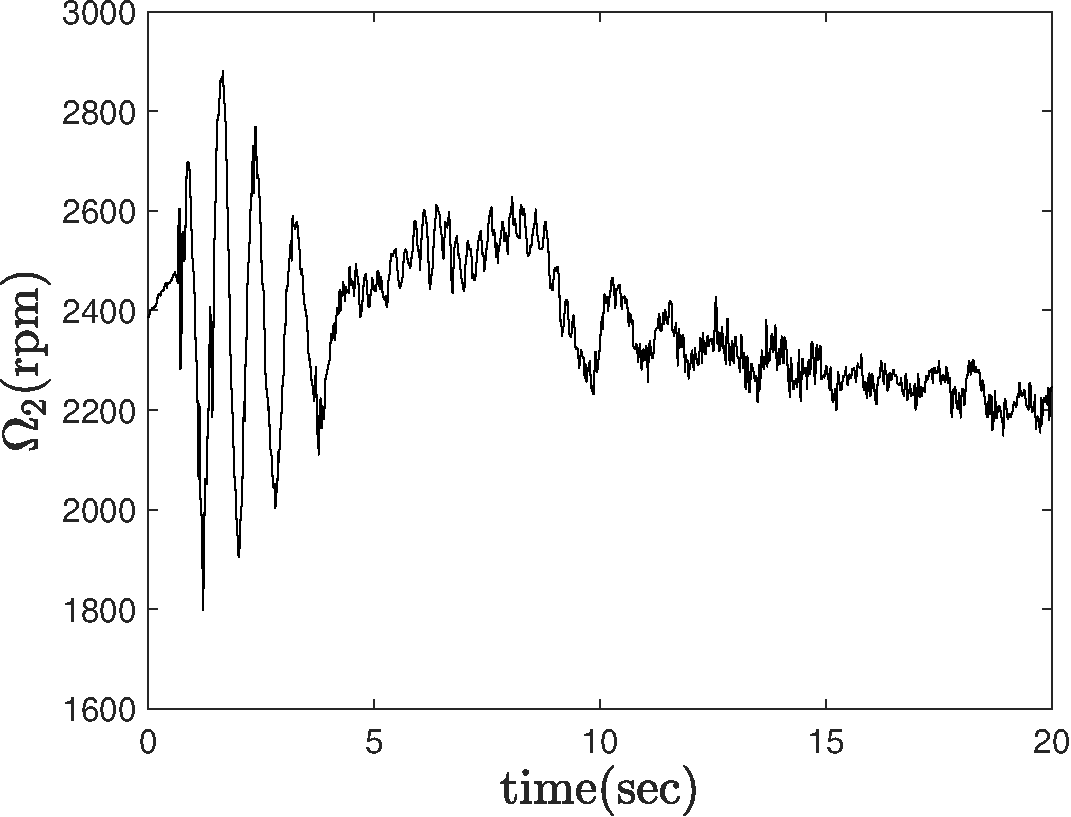
\includegraphics[width=.23\linewidth]{../Figure/implementation/lqidg_Omega_2}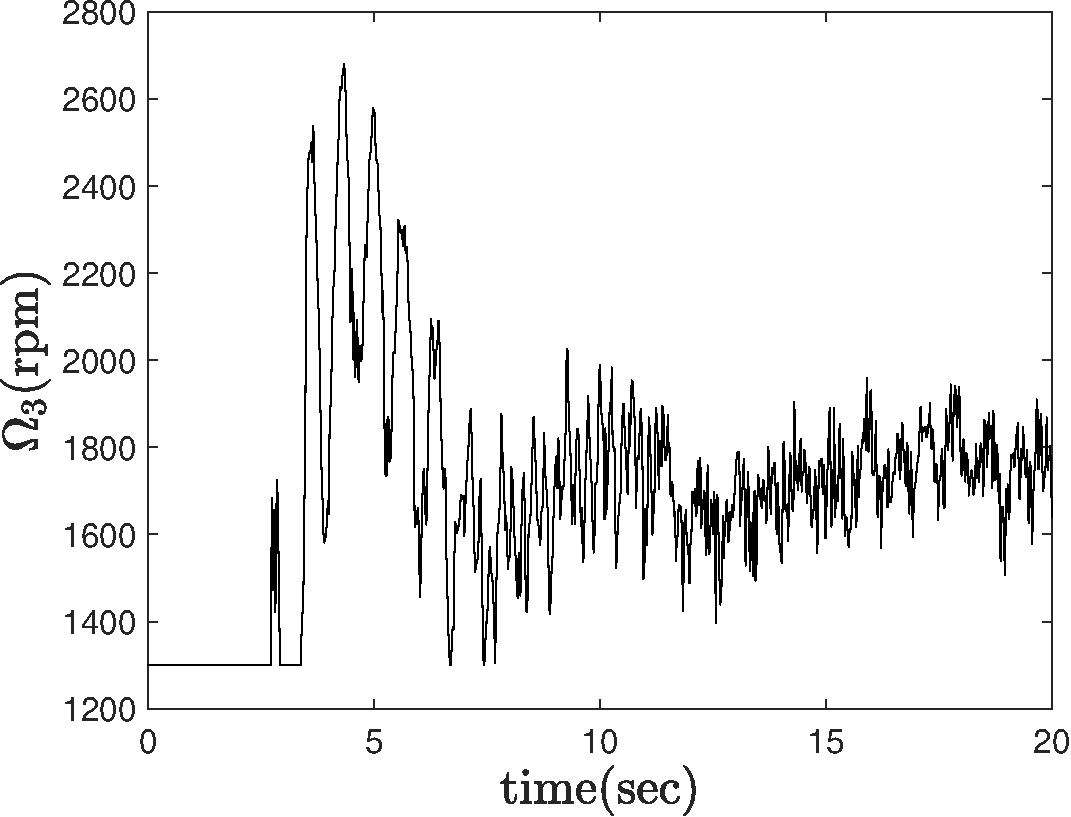
\includegraphics[width=.23\linewidth]{../Figure/implementation/lqidg_Omega_3}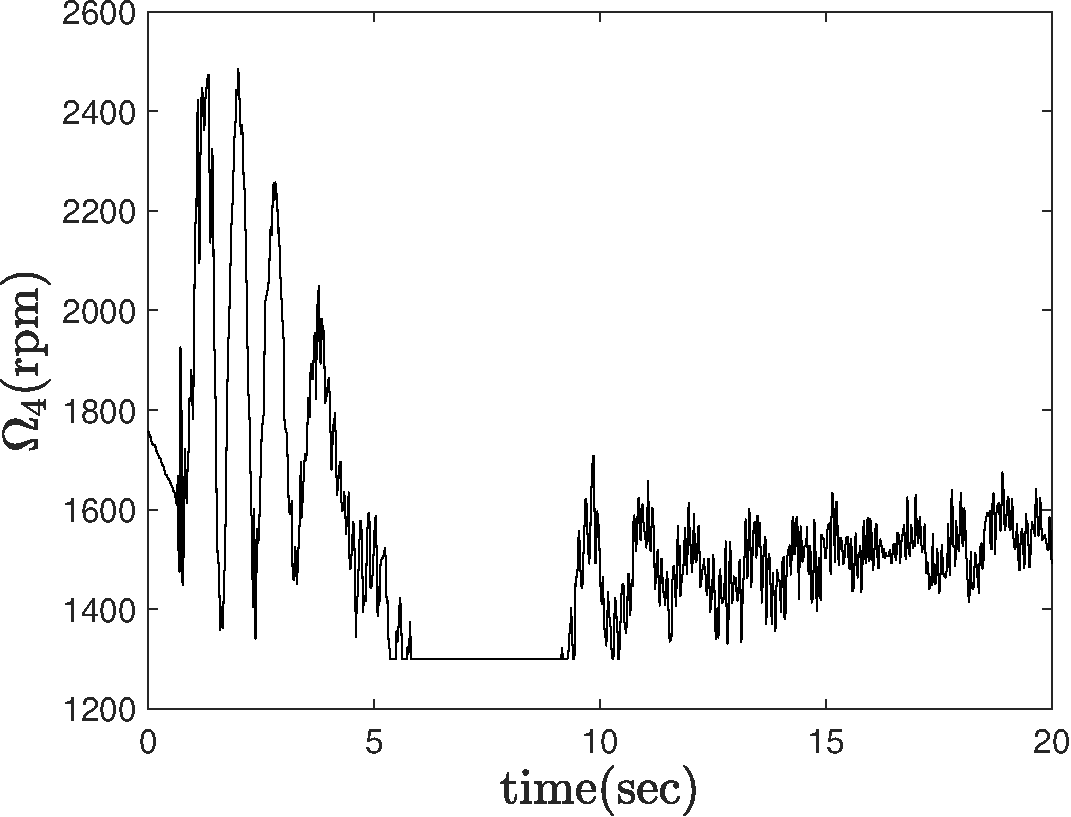
\includegraphics[width=.23\linewidth]{../Figure/implementation/lqidg_Omega_4}
	}
	\hfil
	\subfloat[\label{fig:omega_square}]{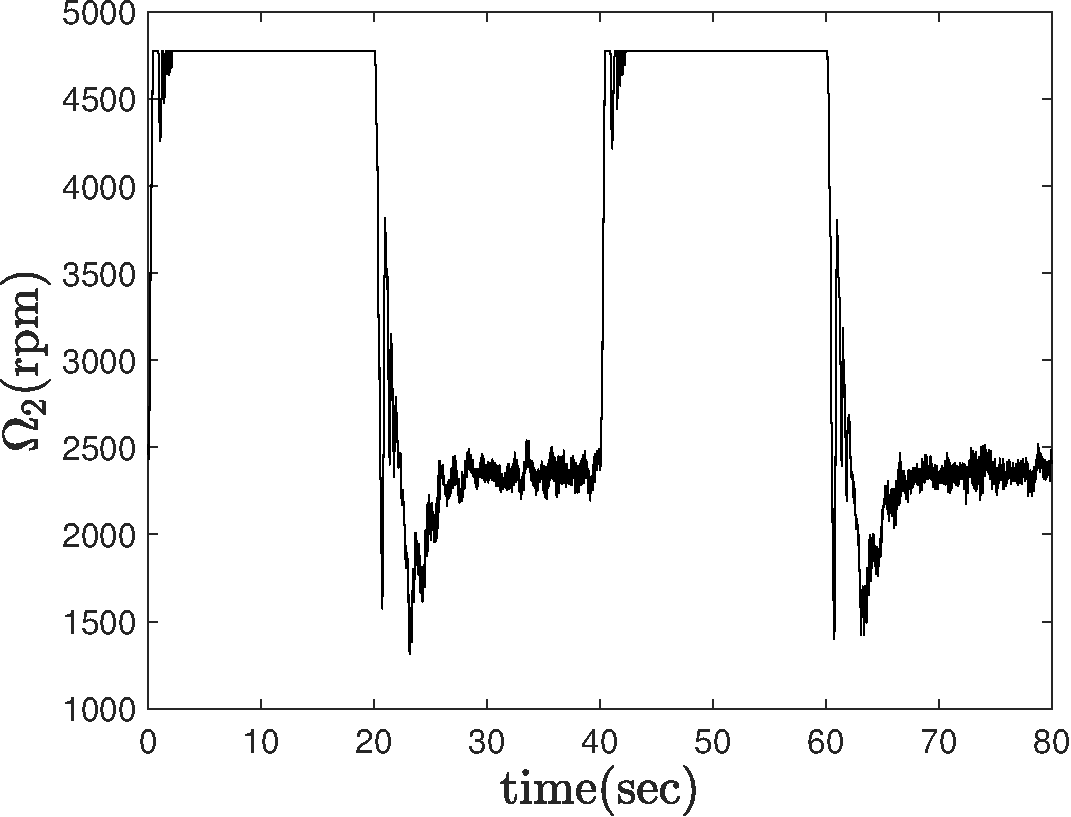
\includegraphics[width=.23\linewidth]{../Figure/implementation/square/lqidg_squre_omega_2}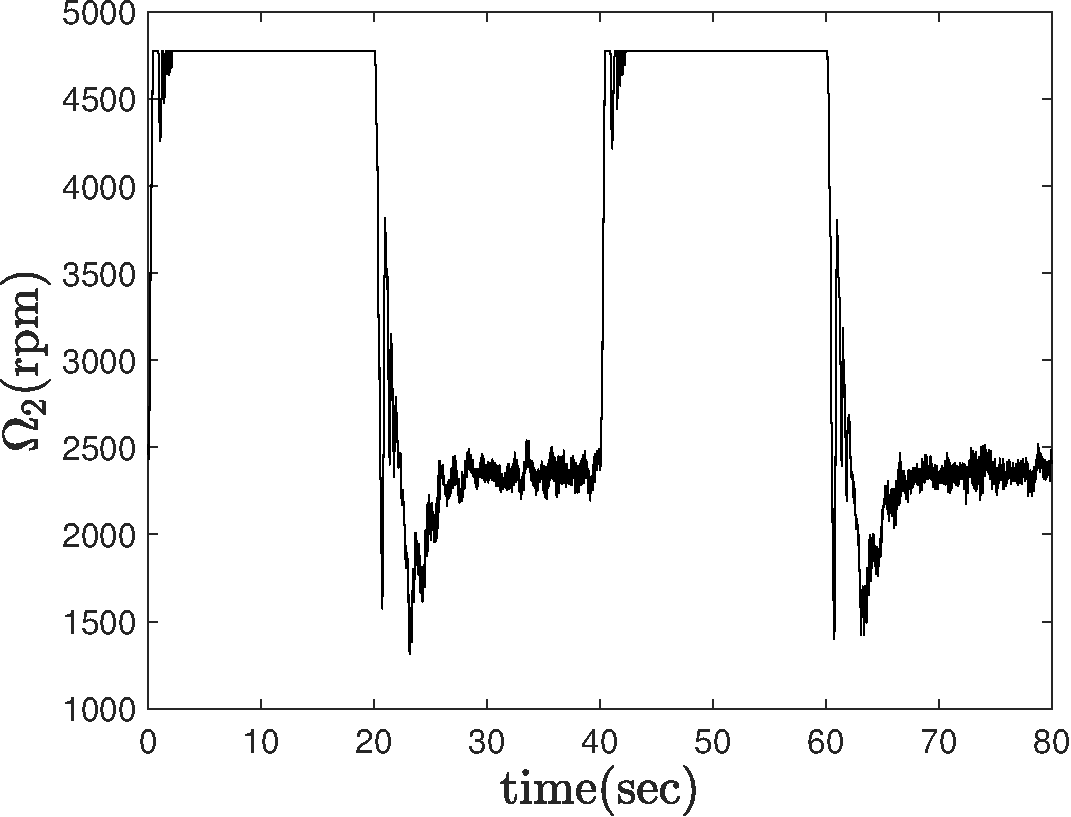
\includegraphics[width=.23\linewidth]{../Figure/implementation/square/lqidg_squre_omega_2}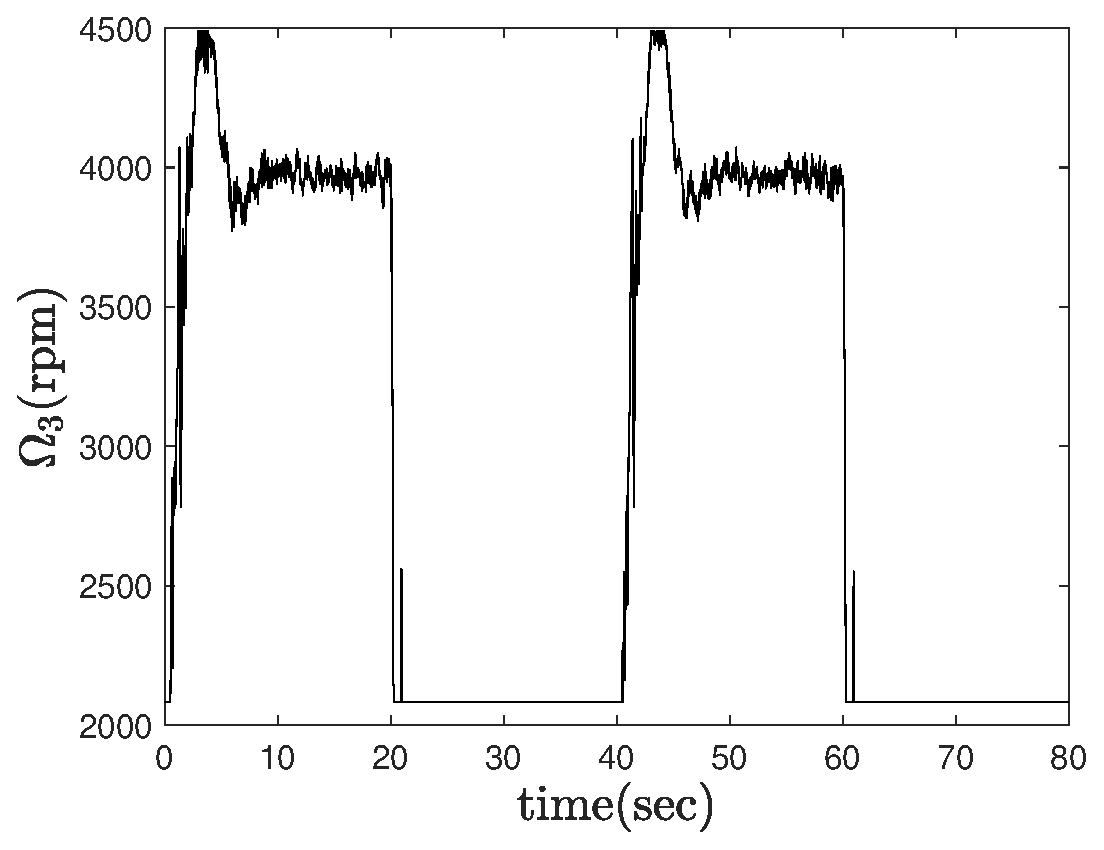
\includegraphics[width=.23\linewidth]{../Figure/implementation/square/lqidg_squre_omega_3}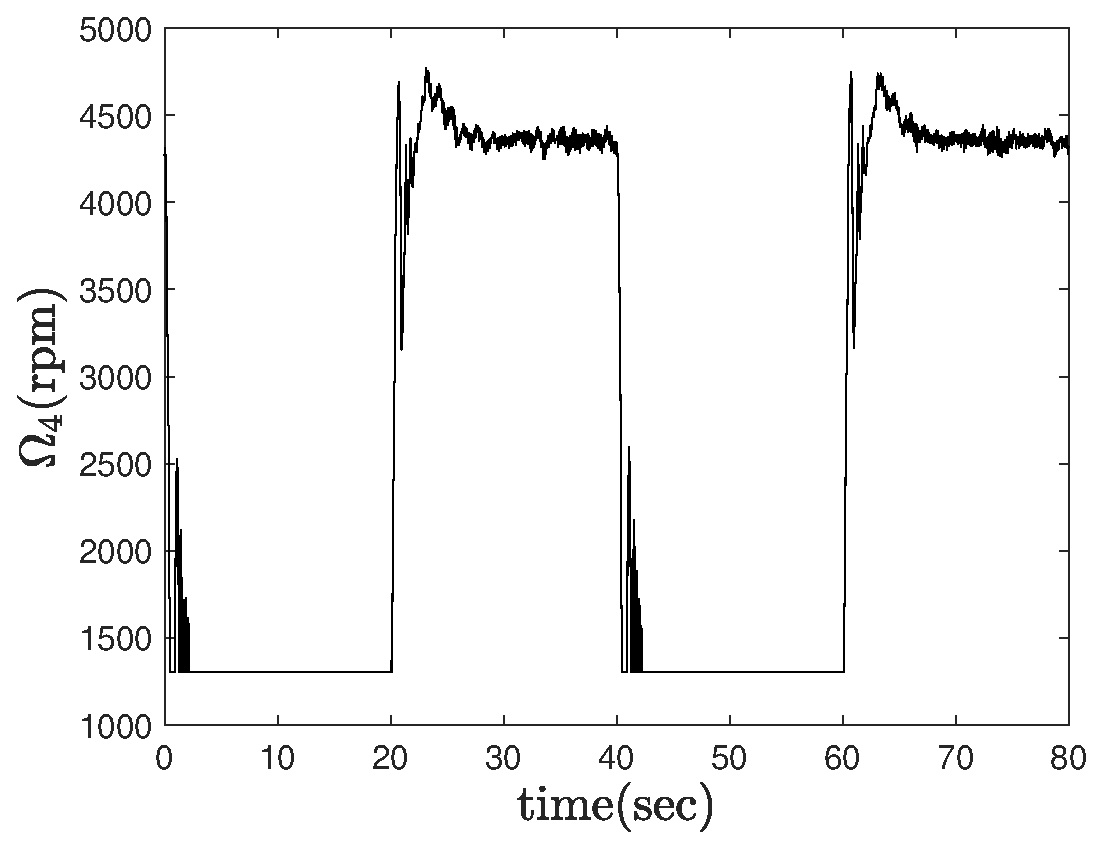
\includegraphics[width=.23\linewidth]{../Figure/implementation/square/lqidg_squre_omega_4}}
	\caption{Temporal Evolution of Angular Velocity Commands for the LQIR-DG Controller}
	\label{fig:omega}
\end{figure}
\subsubsection{Performance of the LQIR-DG in Disturbance Rejection}\label{sec:disturbance}
\noindent The performance of the proposed controller in the input disturbance is shown in Figure \ref{fig:disturbance}. The input disturbance, $\mathrm{d\Omega_i}$, is considered as a change in the command of the rotational velocity, modeled as:
\begin{equation}
	\mathrm{d\Omega_1} = \mathrm{d\Omega_2} = -\mathrm{d\Omega_3} = -\mathrm{d\Omega_4} = \begin{cases}
		500_{\mathrm{rpm}} \quad &20<t<60\\
		0 \quad &\mathrm{other}
	\end{cases}
\end{equation}
Figure \ref{fig:disturbance} \ref{sub@fig:disturbance_angle} illustrate the desired and the actual roll and pitch angles in the regulation problem. The results indicate that the LQIR-DG controller can stabilize the quadrotor platform when the input disturbance is present.
\begin{figure}[H]
	\centering
	\subfloat[\label{fig:disturbance_angle}]{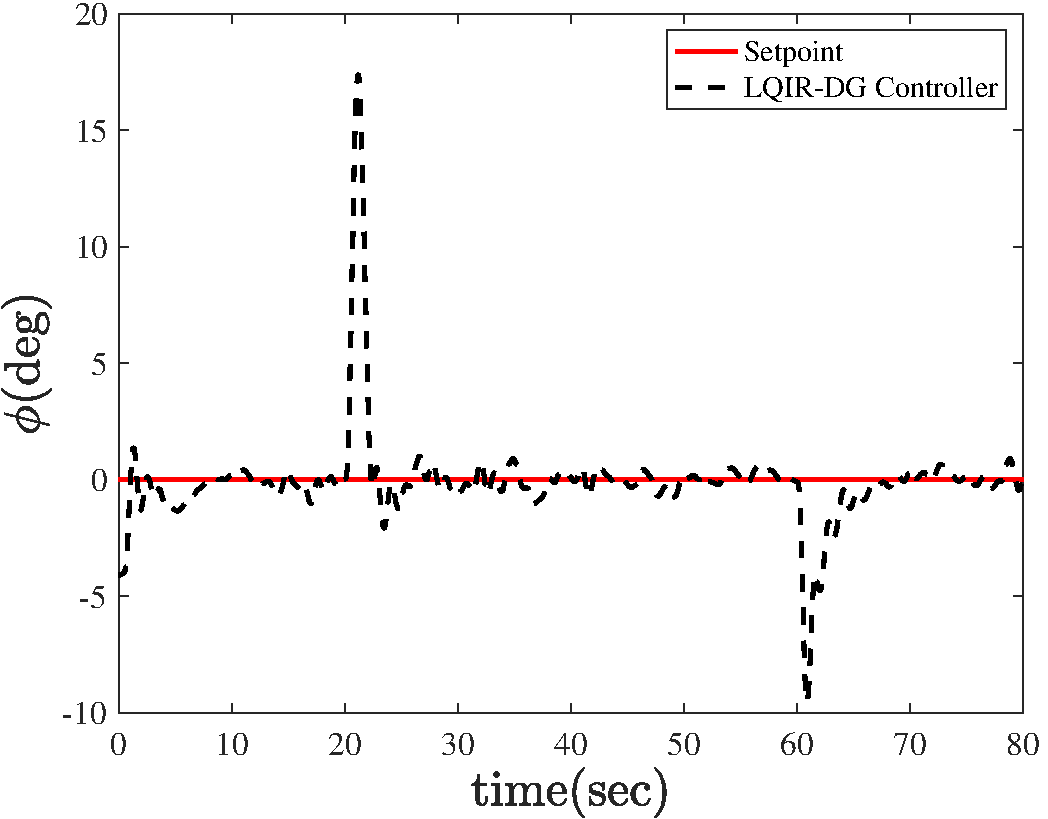
\includegraphics[width=.49\linewidth]{../Figure/implementation/disturbance/lqidg_roll}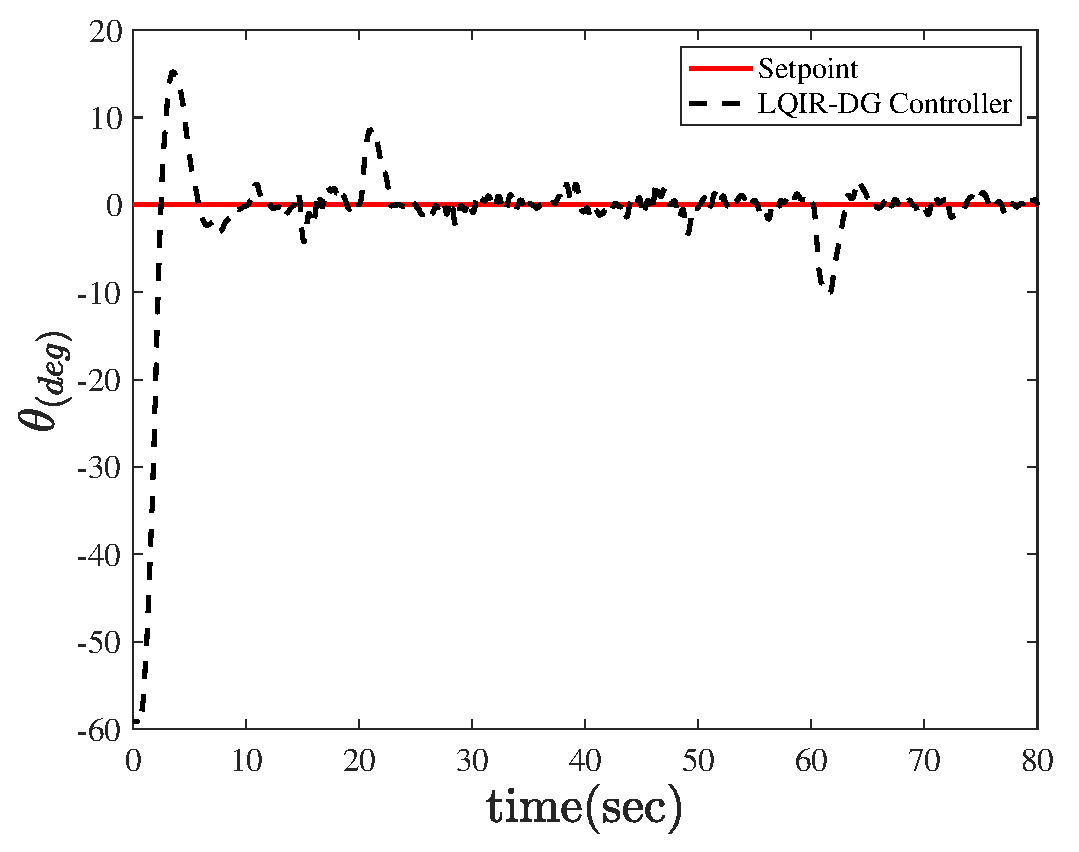
\includegraphics[width=.49\linewidth]{../Figure/implementation/disturbance/lqidg_pitch}
	}
	\caption{Comparison of the desired and actual roll and pitch angle in the presence of the input disturbance.}
	\label{fig:disturbance}
\end{figure}
\subsubsection{Investigating the Impact of Modeling Uncertainty}\label{sec:model-uncertainty}
\noindent In this section, the performance of the LQIR-DG controller is investigated while considering uncertainty in the 3DoF experimental model. 
To achieve this, 50 and 100 grams were added to the roll and pitch axes, respectively, as shown in Figure \ref{fig:quadrotor_with_weight}.
Figure \ref{fig:weight} \ref{sub@fig:weight_roll} compares the desired and the actual roll angle and Figure \ref{fig:weight} \ref{sub@fig:weight_pitch} shows the desired and the actual pitch angle when the uncertainty of moments of inertia is presented.
Moreover, Figure \ref{fig:weight} \ref{sub@fig:omega_weight} shows the rotational velocity command of the experimental platform in the presence of model uncertainty.
The implementation results indicate that the LQIR-DG controller converges to the desired values in the presence of the modeling uncertainty.
\begin{figure}[H]
	\centering
	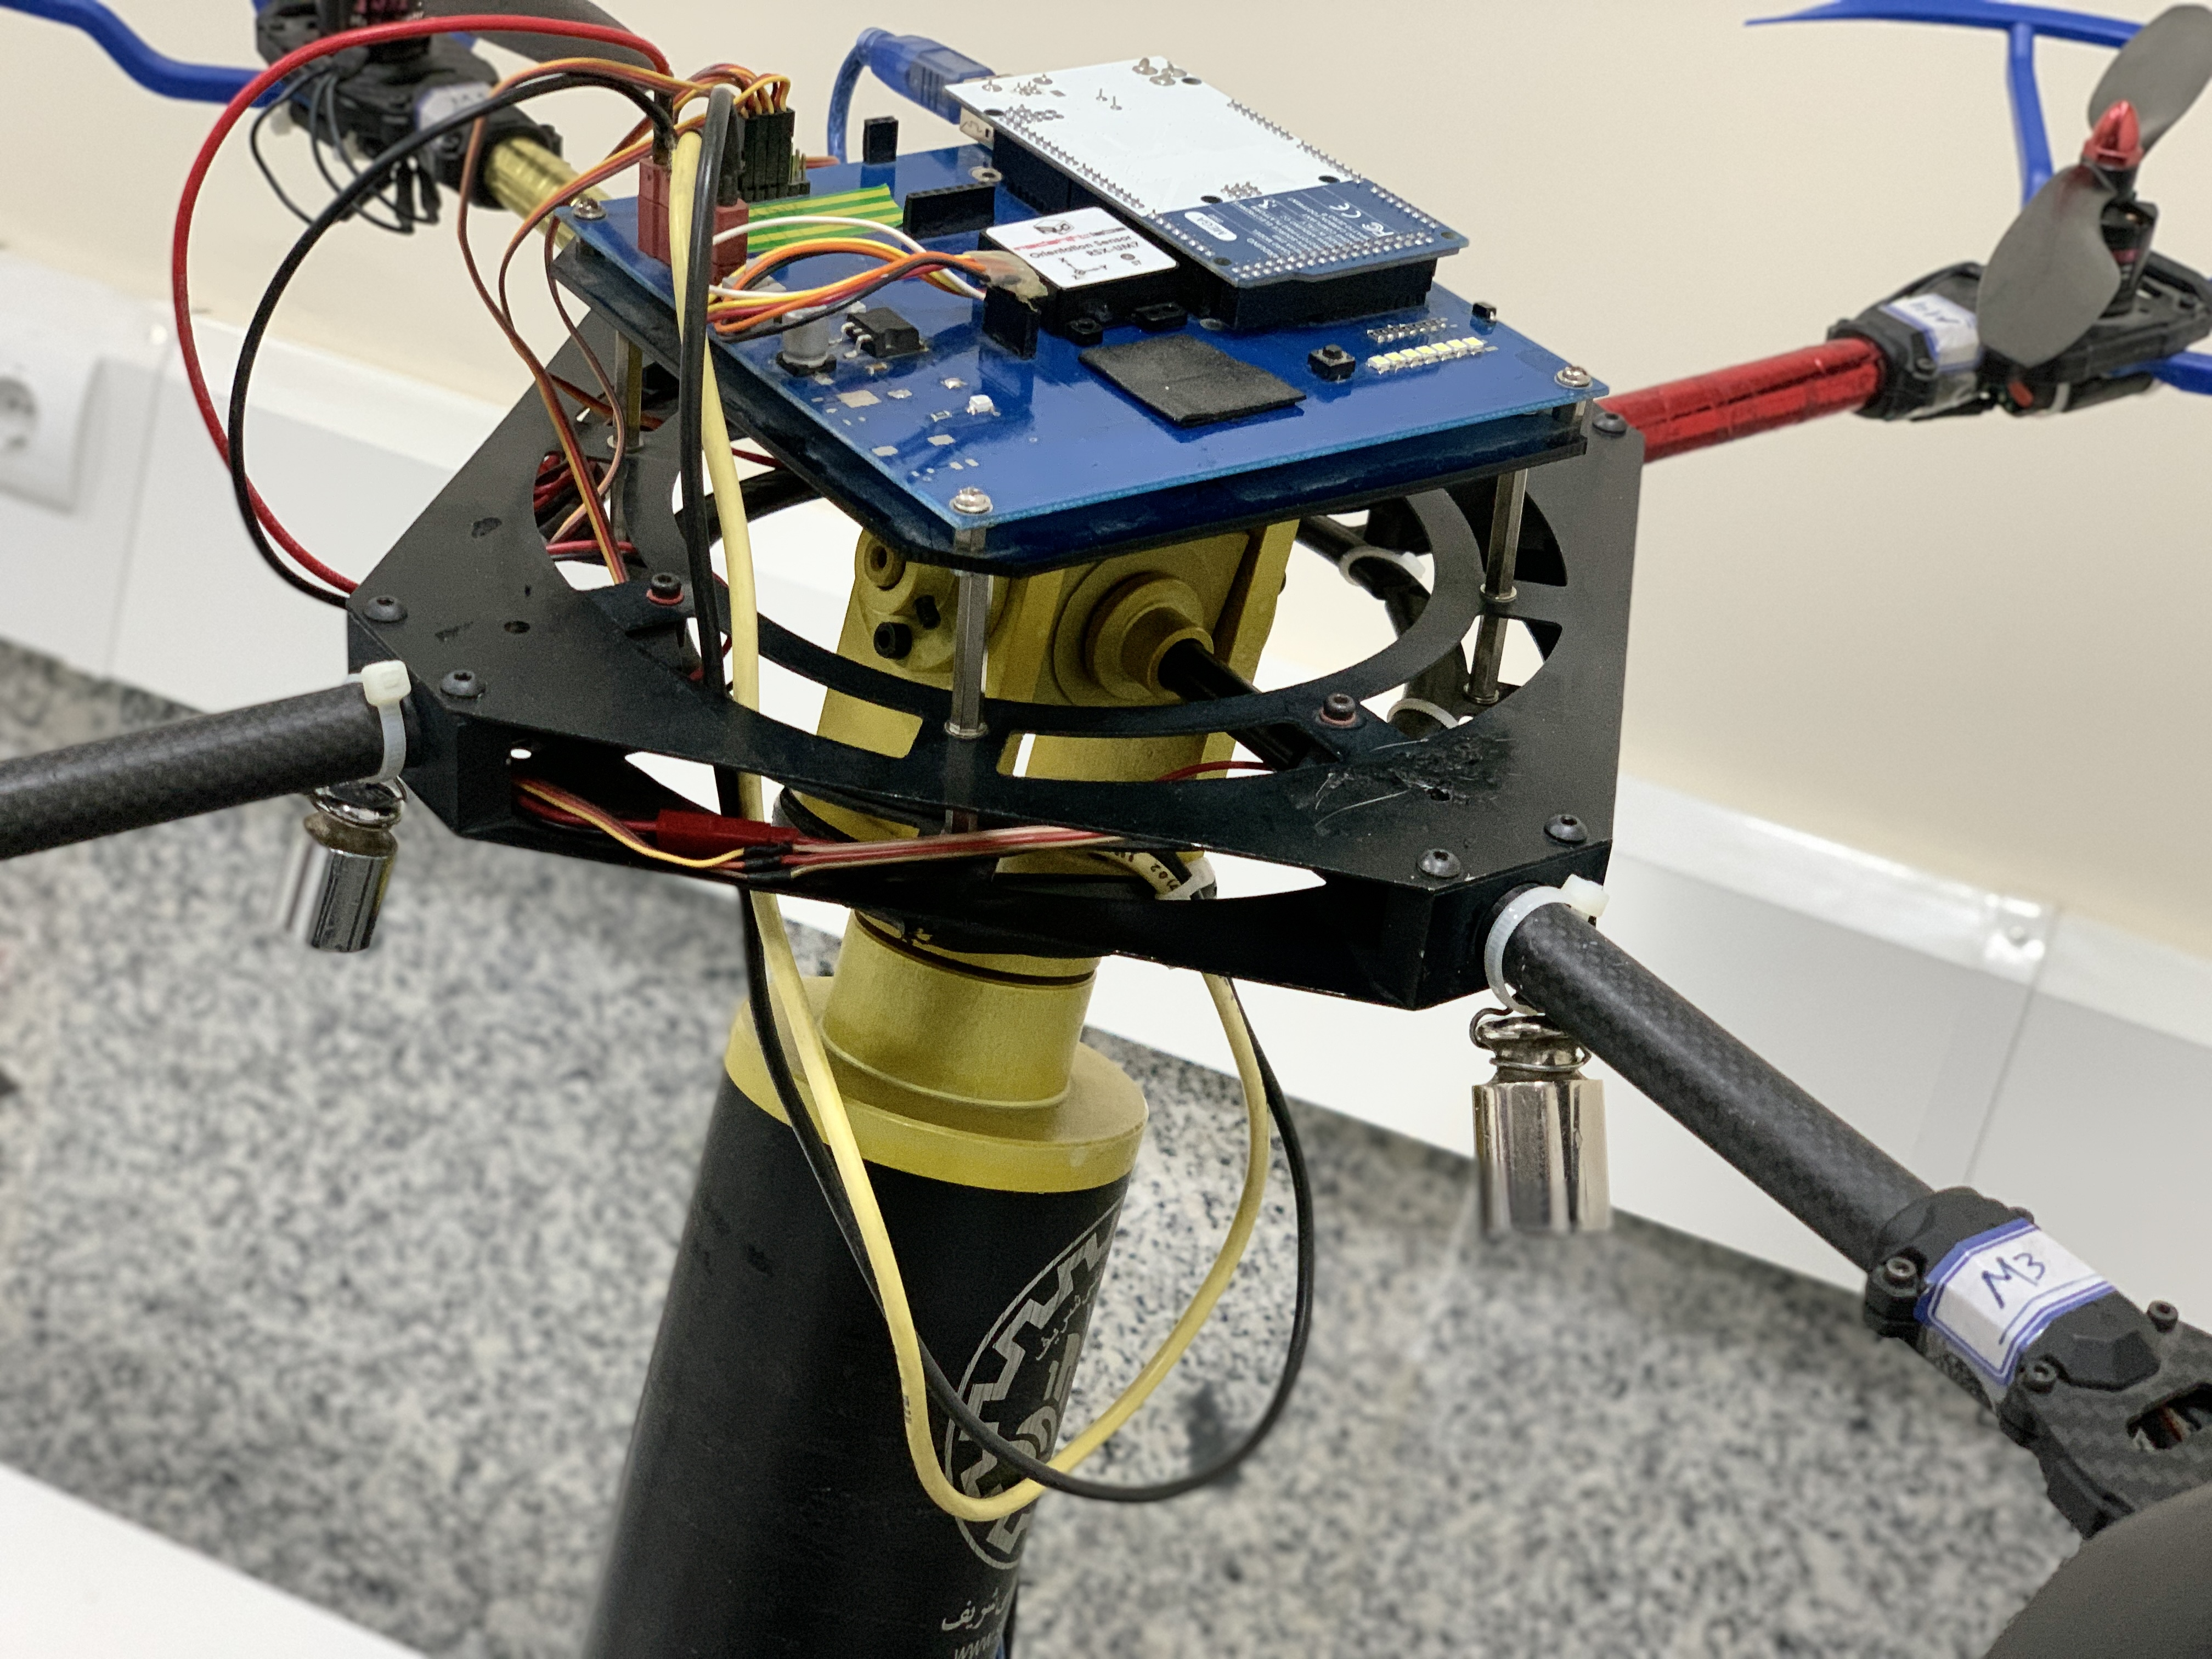
\includegraphics[width=0.49\textwidth]{../Figure/implementation/weight/Quad_with_weight.jpg}
	\caption{Quadrotor 3DoF Platform with Added Weight.}
	\label{fig:quadrotor_with_weight}
 \end{figure}
 \begin{figure}[H]
	\centering
	\subfloat[\label{fig:weight_roll}]{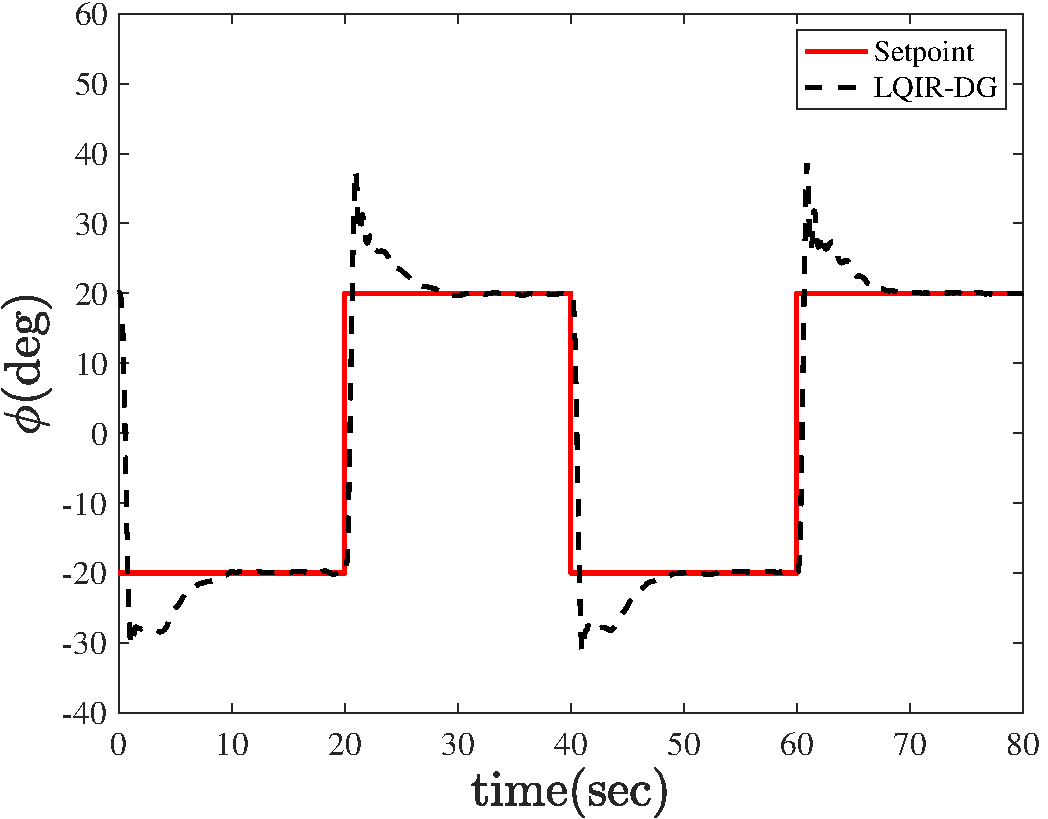
\includegraphics[width=.49\linewidth]{../Figure/implementation/weight/lqidg_roll_20}}\subfloat[\label{fig:weight_pitch}]{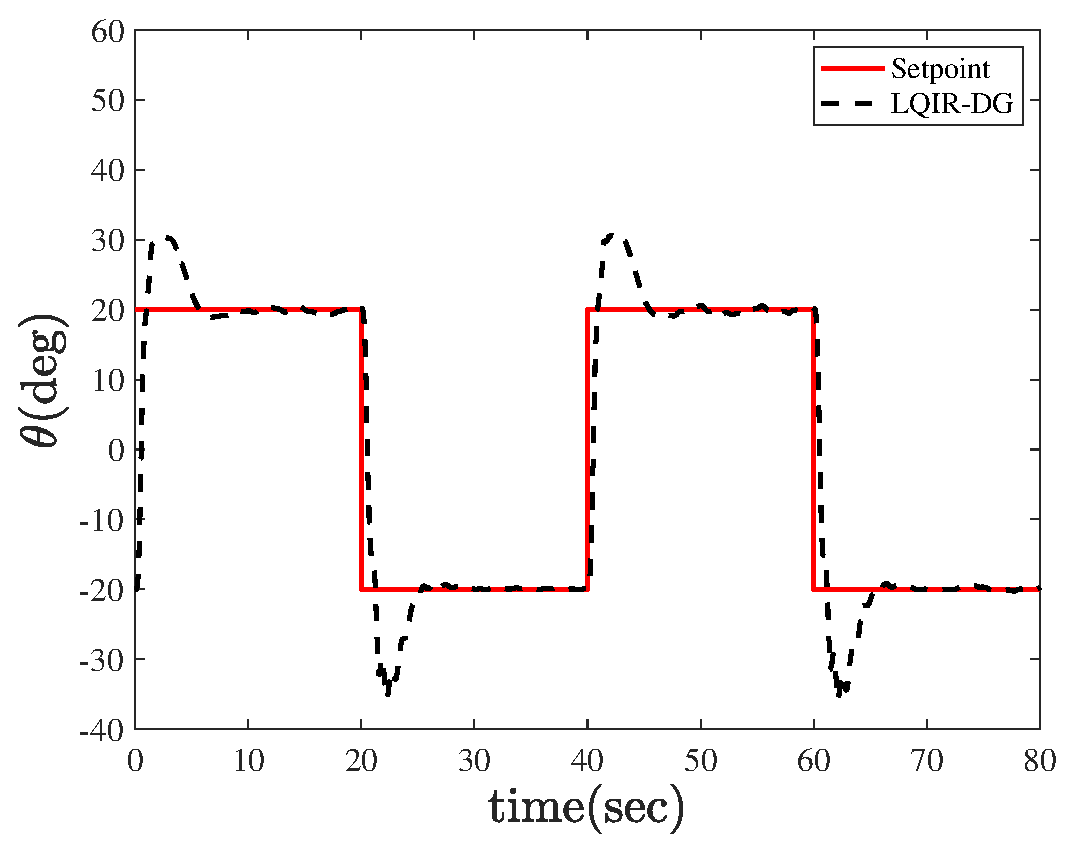
\includegraphics[width=.49\linewidth]{../Figure/implementation/weight/lqidg_pitch_20}
	}
	\hfill
	\subfloat[\label{fig:omega_weight}]{\includegraphics[width=.23\linewidth]{../Figure/implementation/weight/lqidg_Omega_1}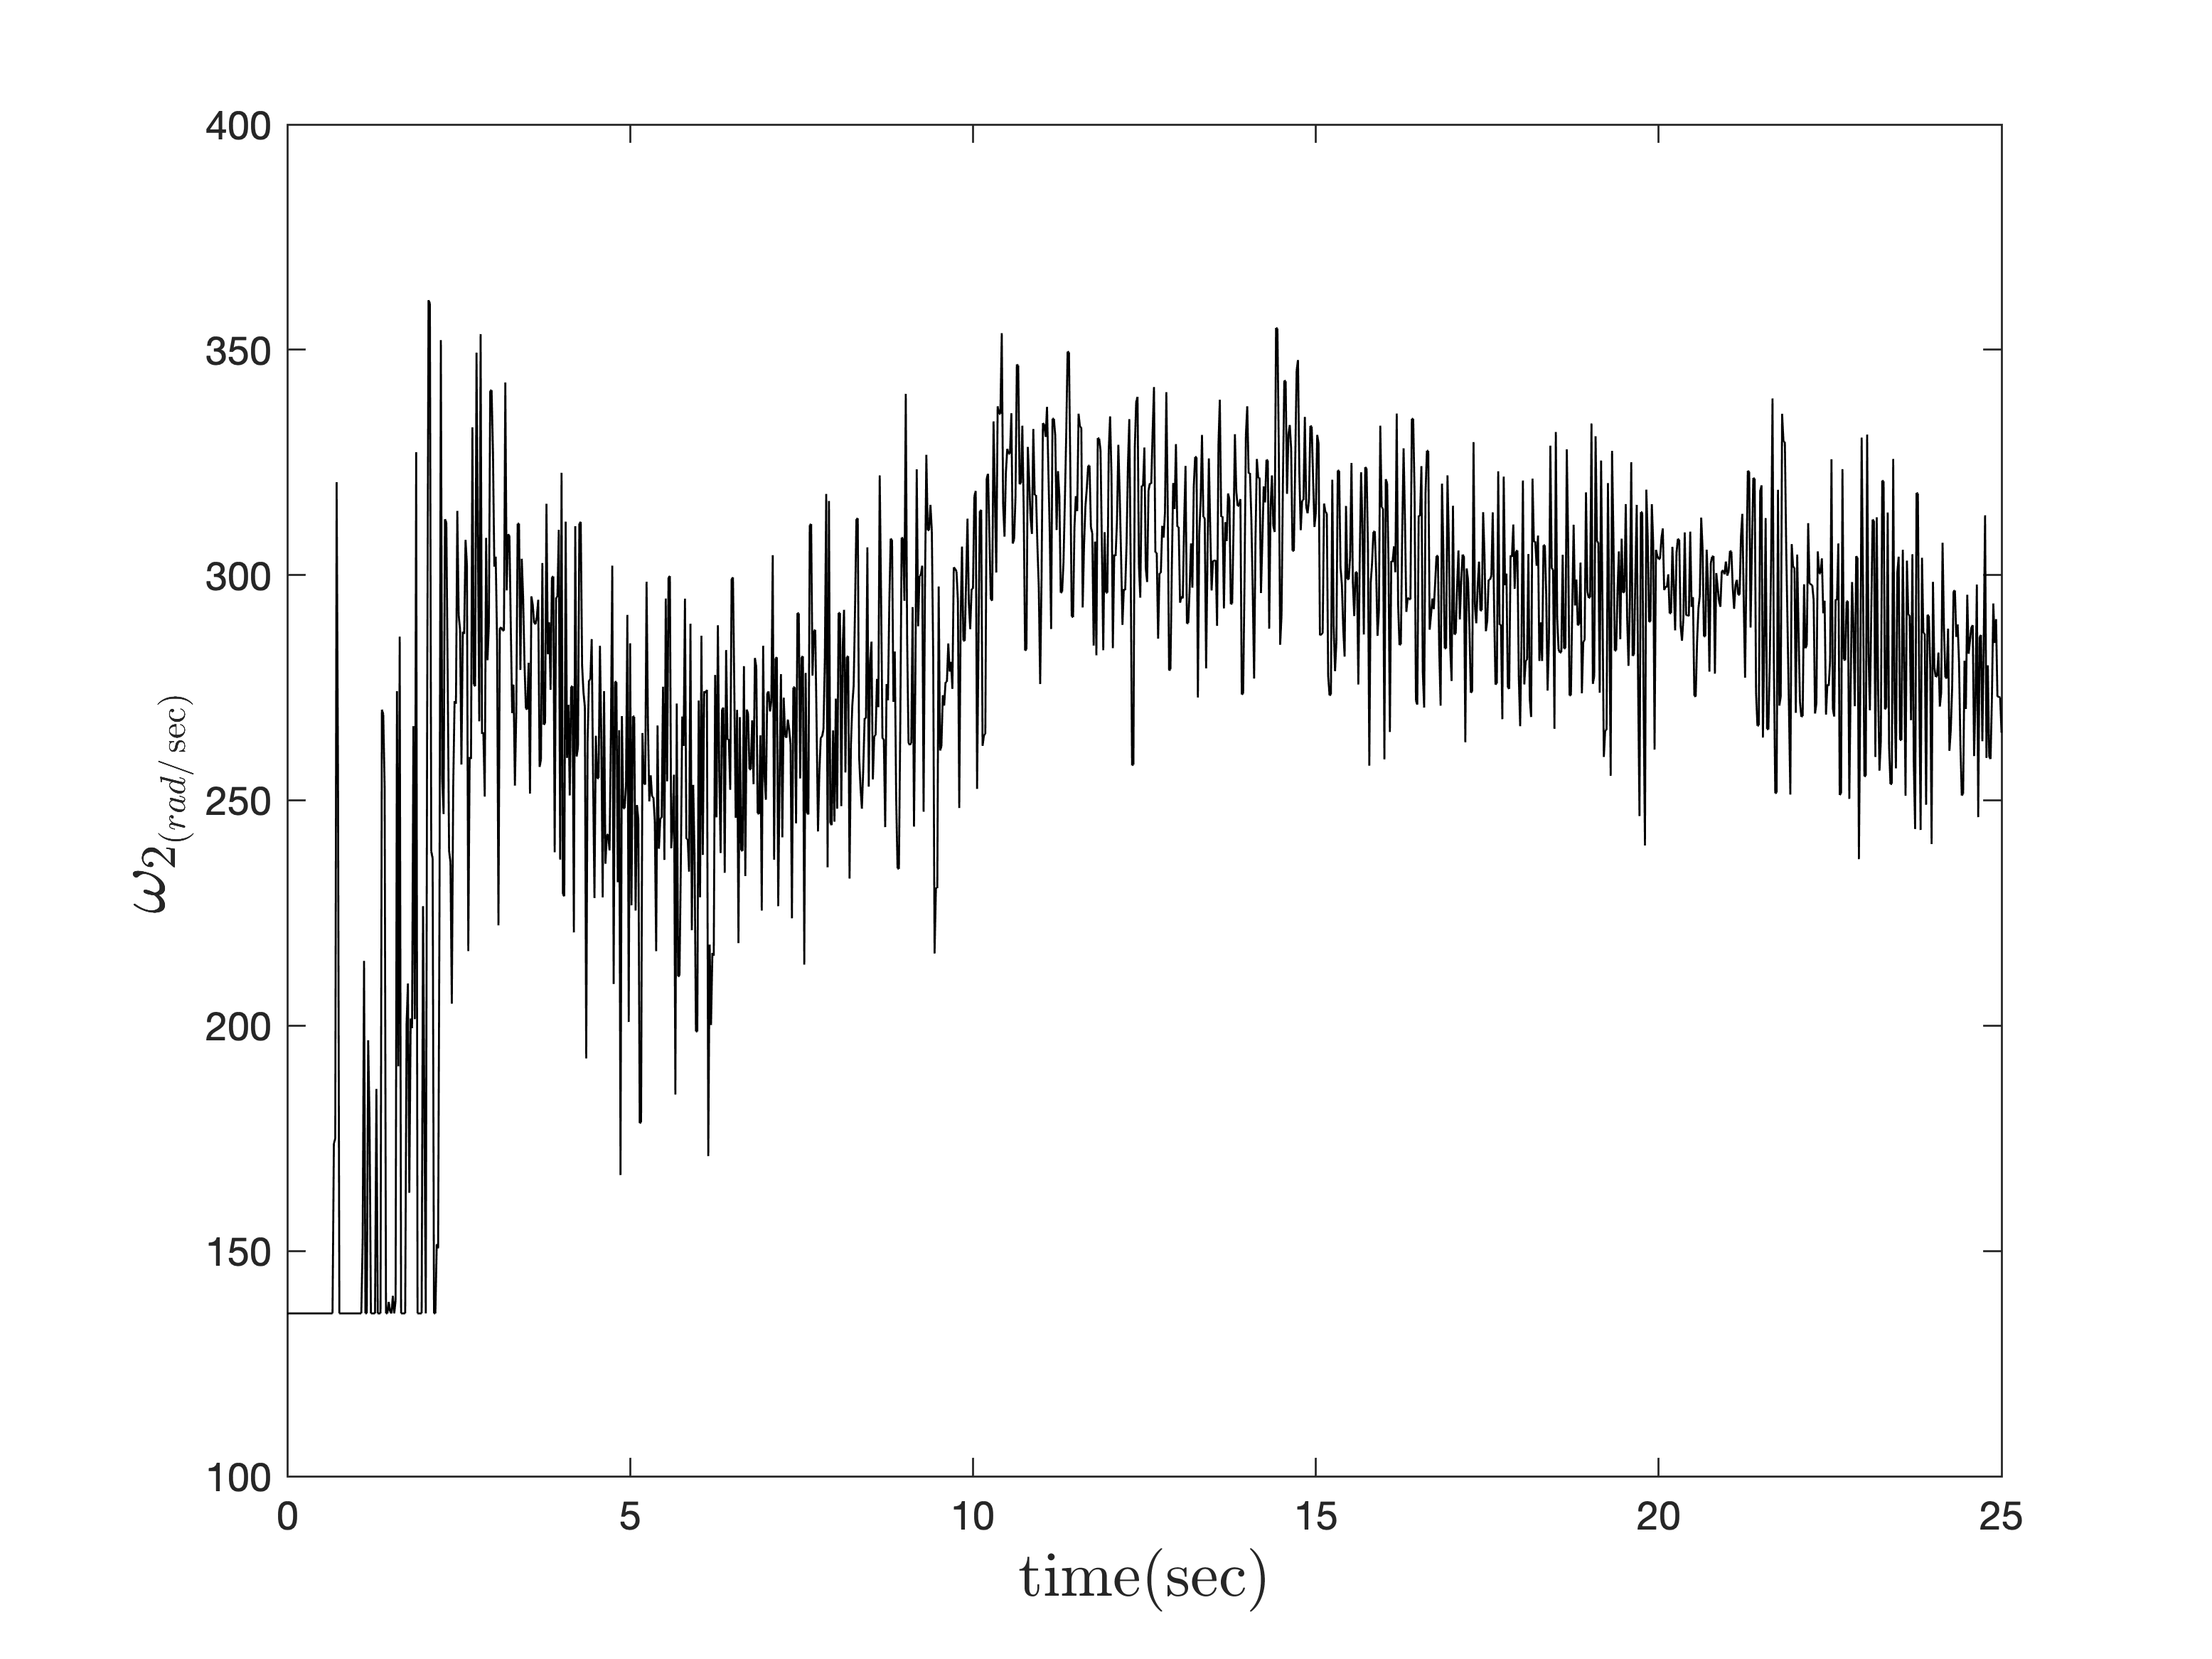
\includegraphics[width=.23\linewidth]{../Figure/implementation/weight/lqidg_Omega_2}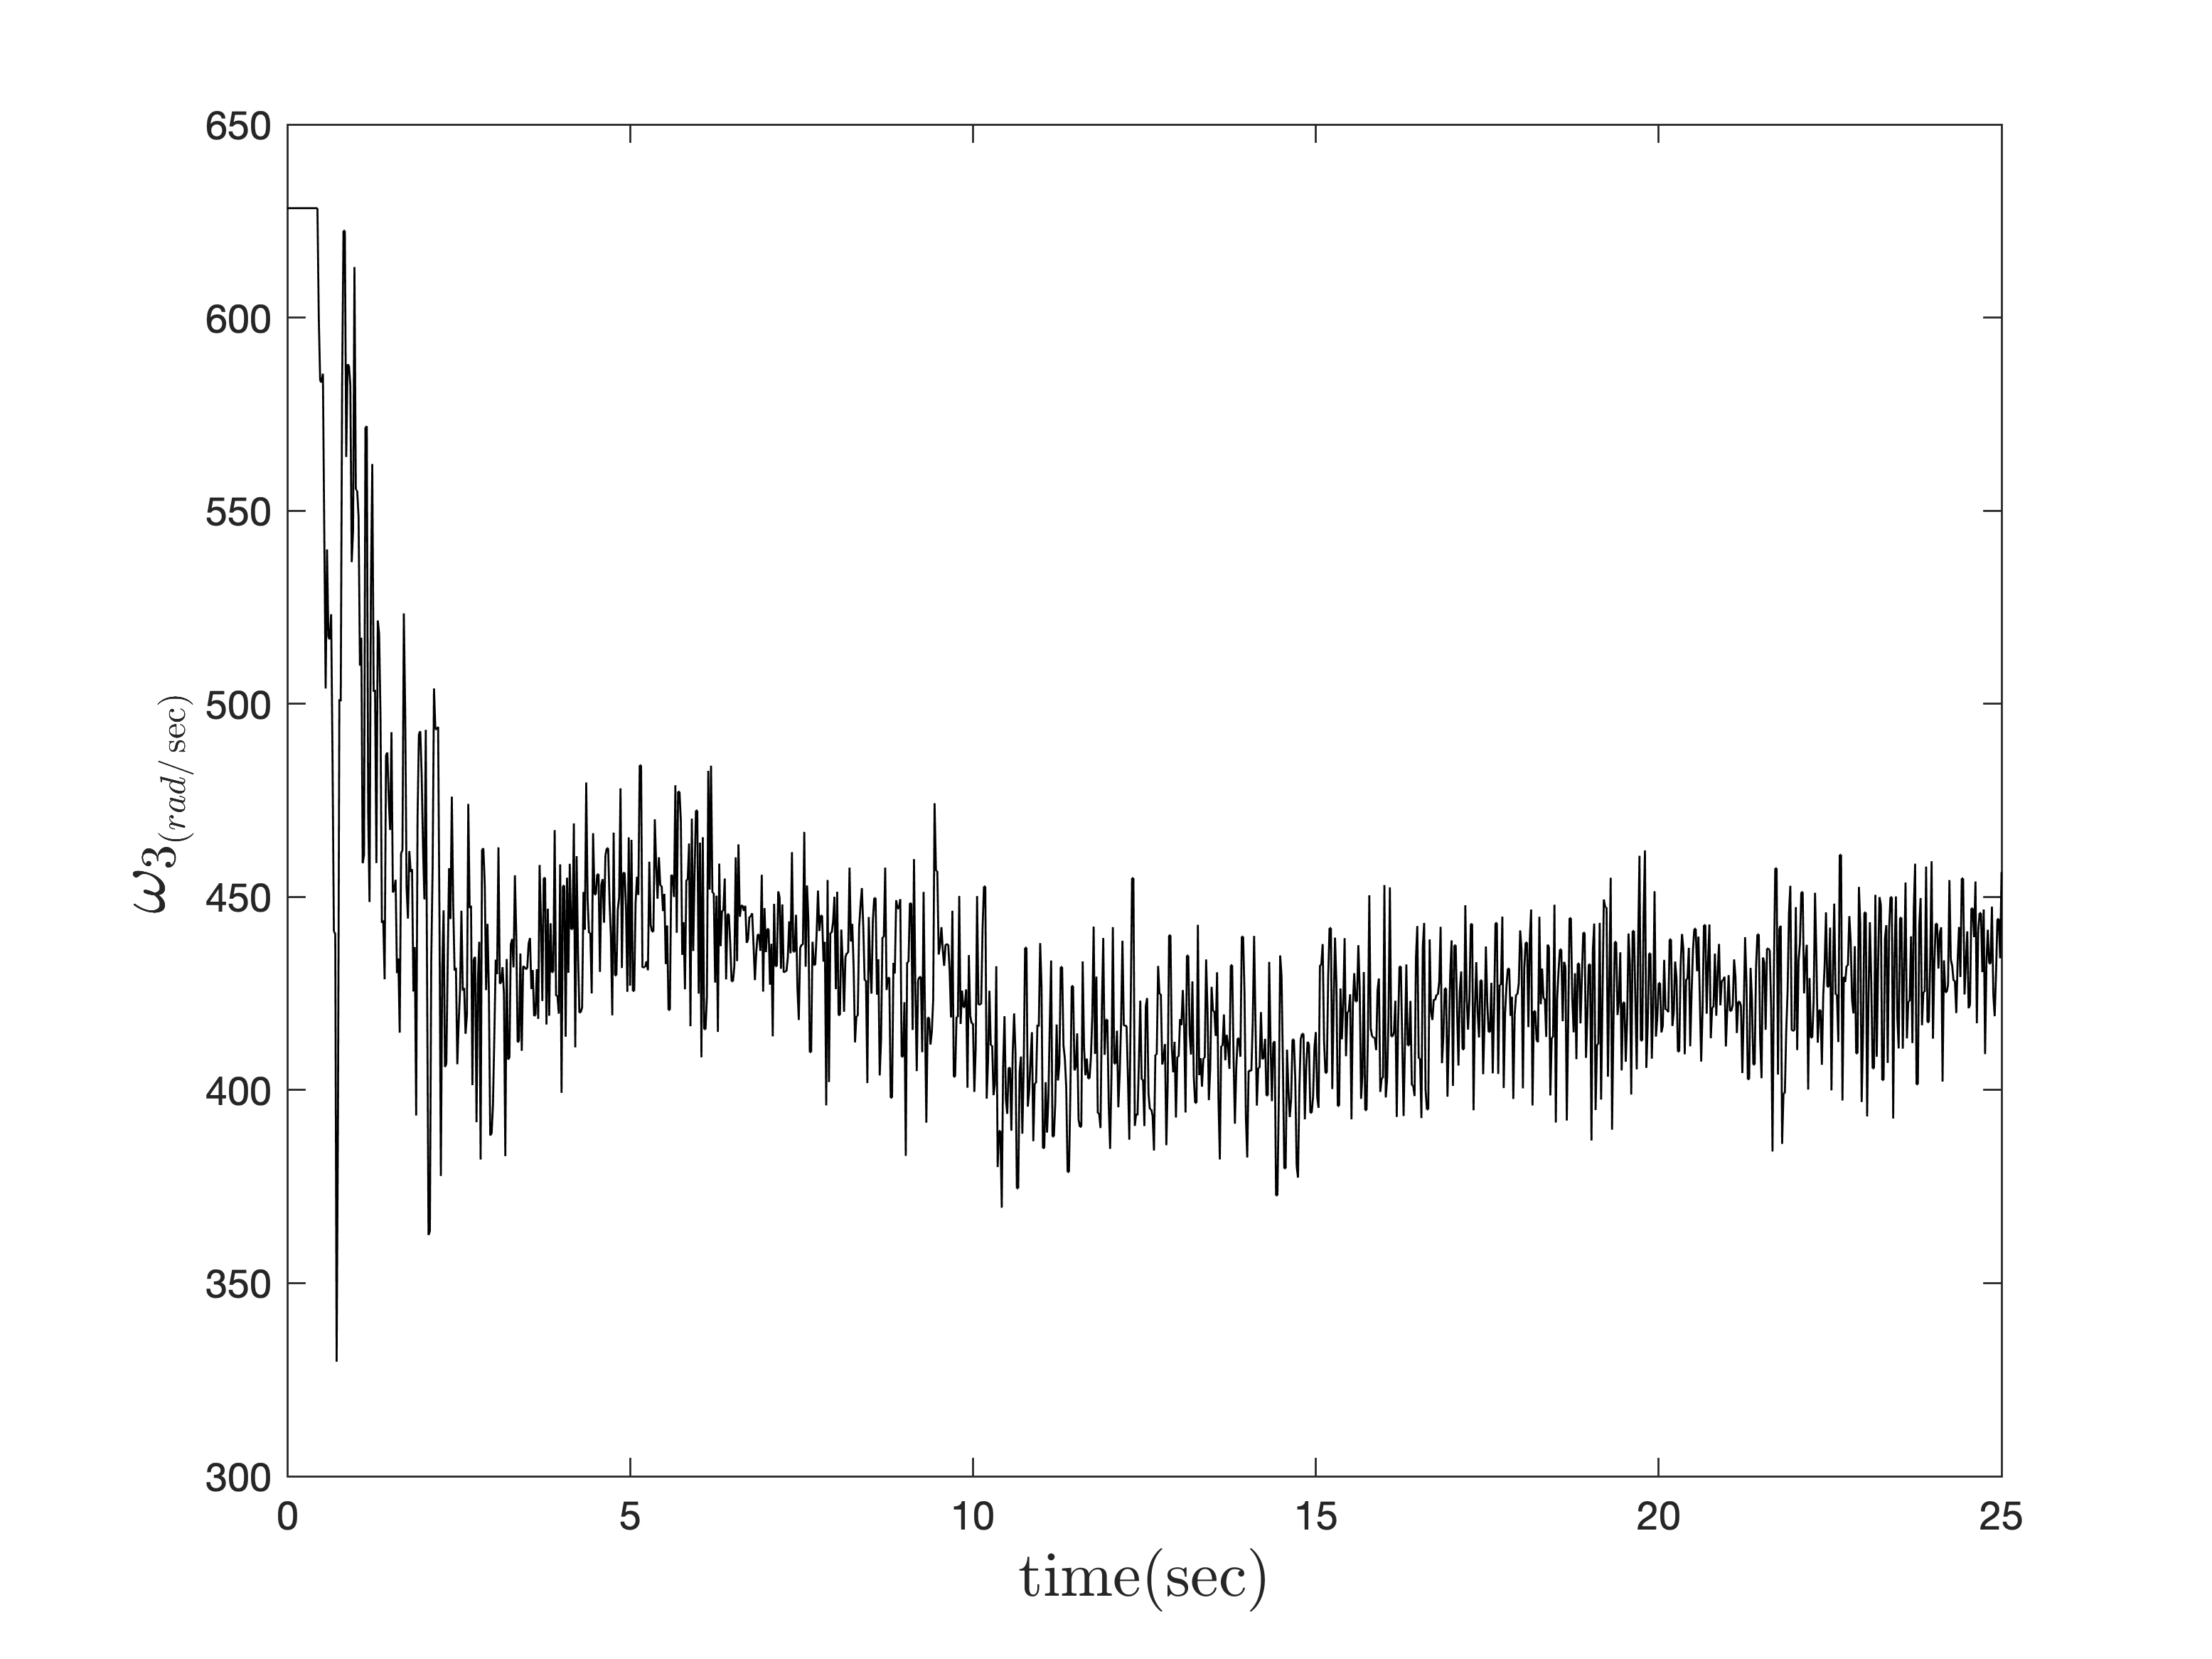
\includegraphics[width=.23\linewidth]{../Figure/implementation/weight/lqidg_Omega_3}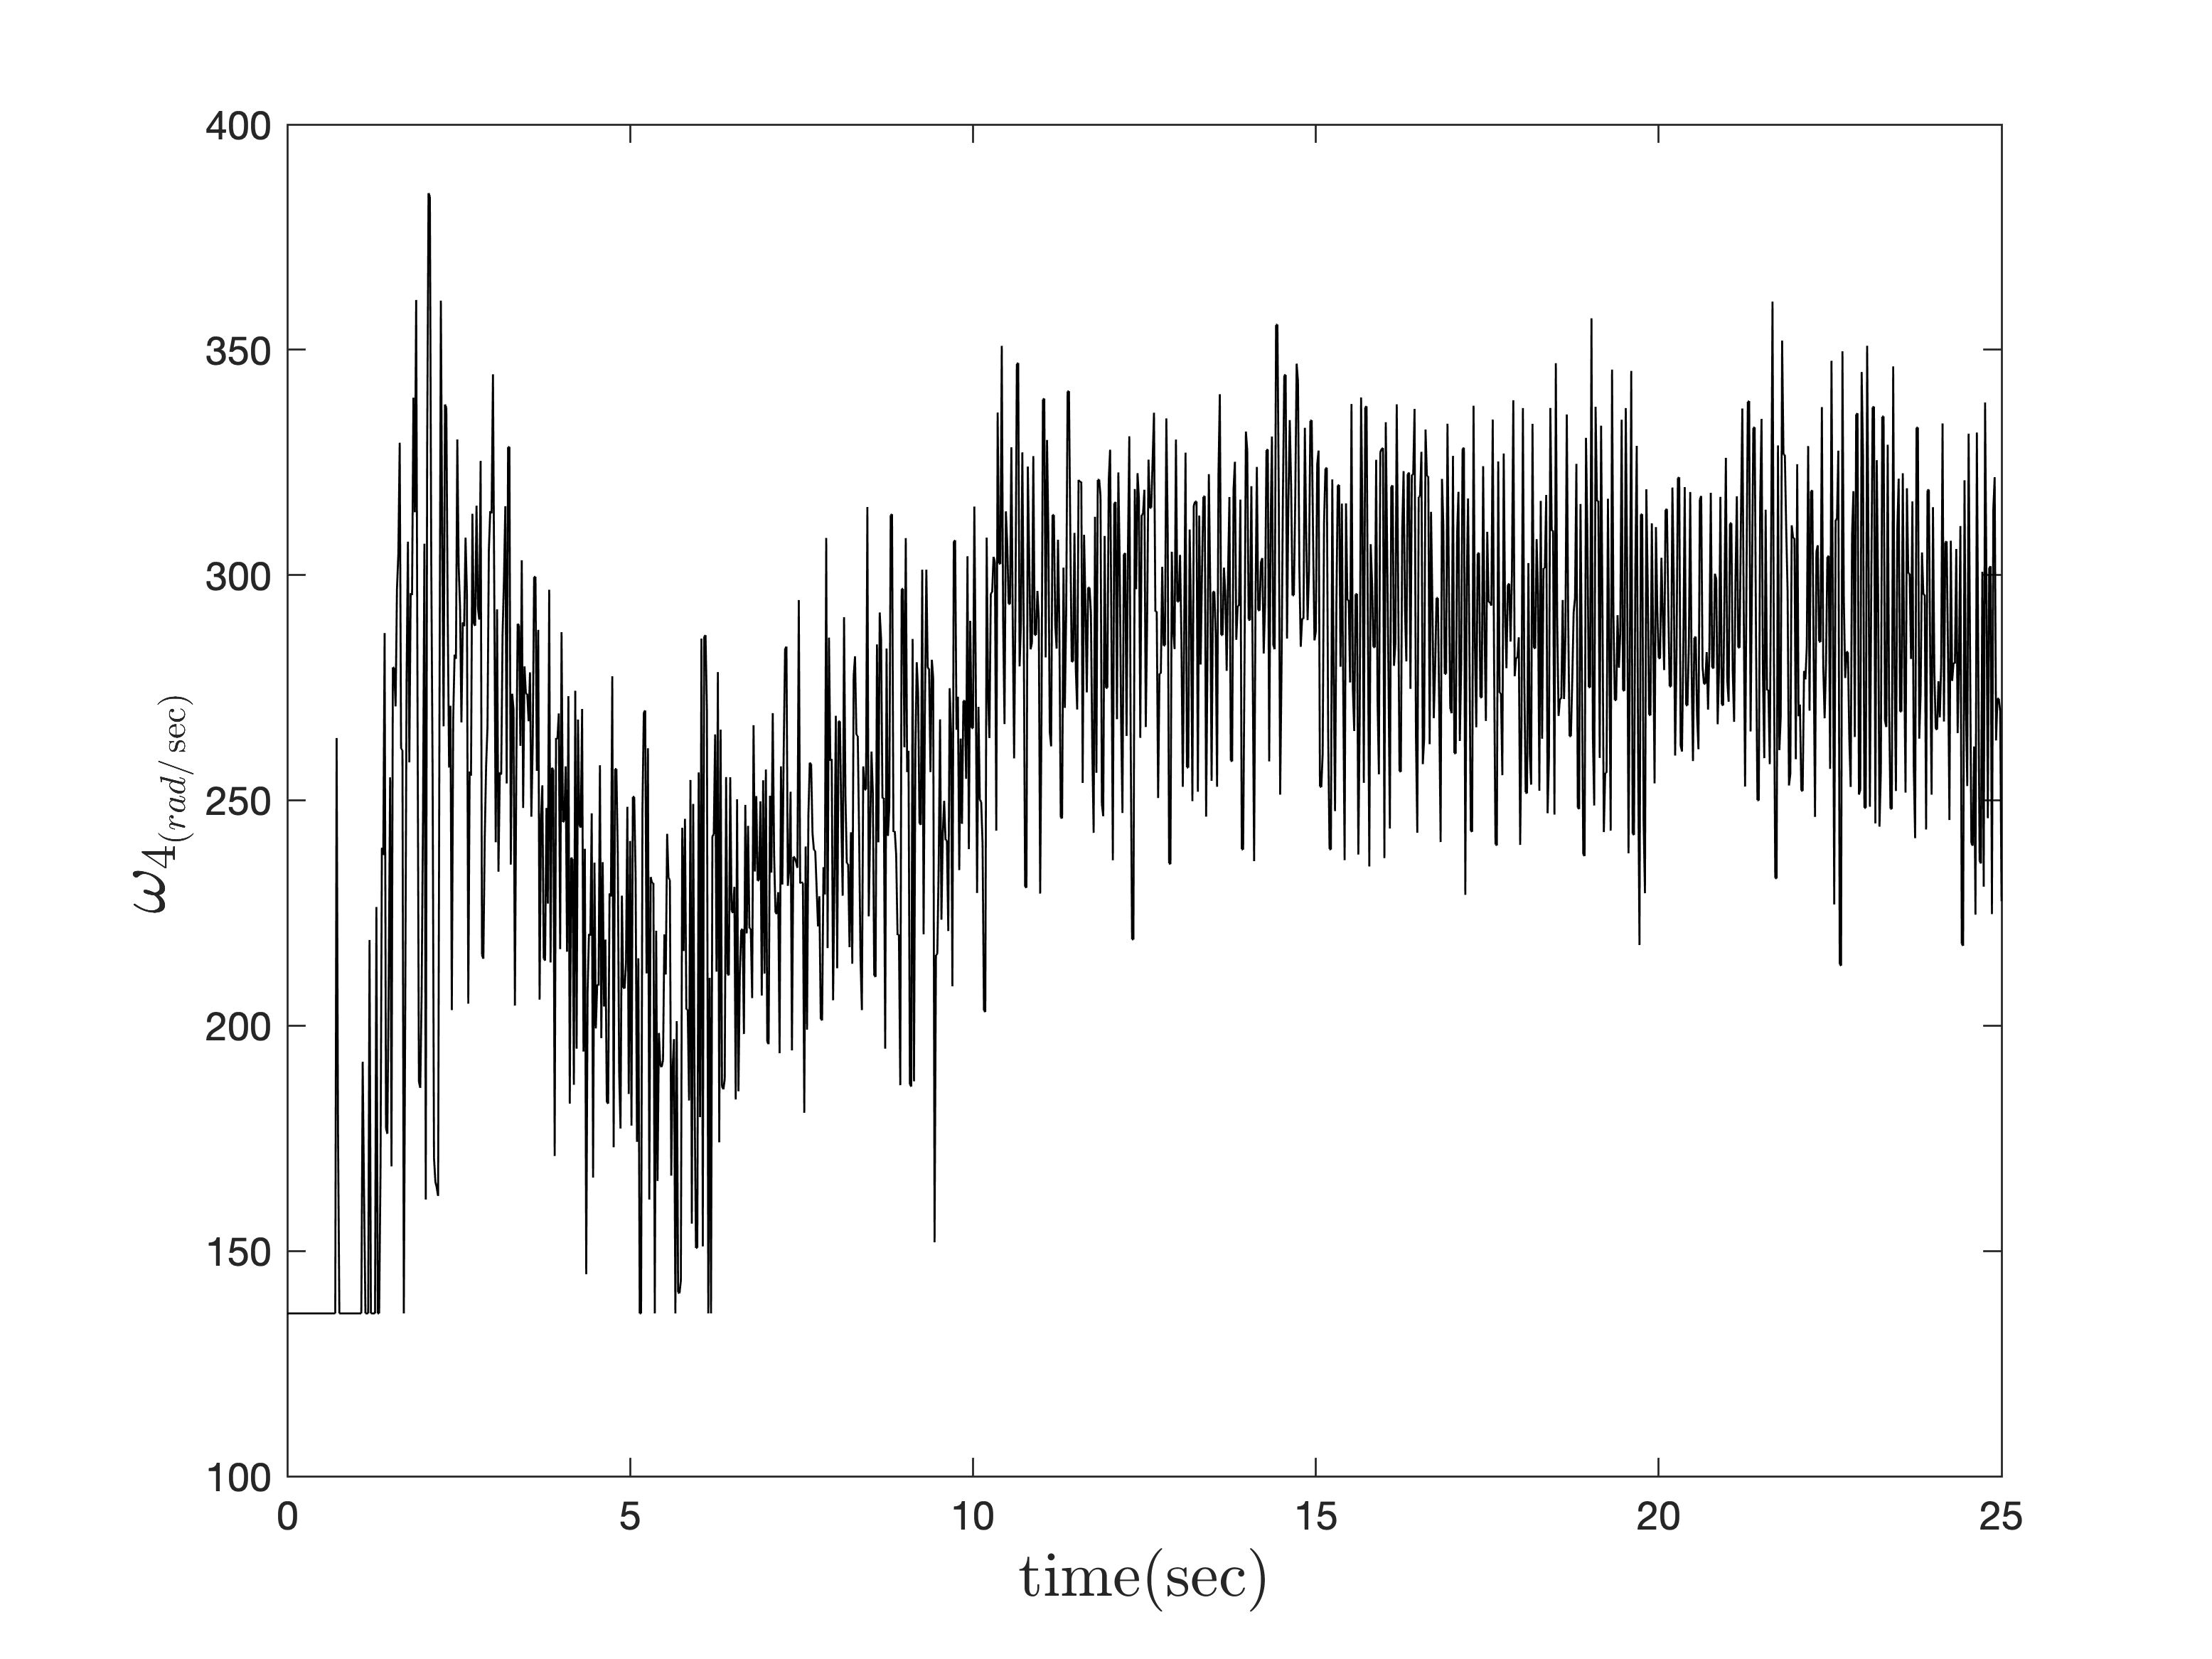
\includegraphics[width=.23\linewidth]{../Figure/implementation/weight/lqidg_Omega_4}}
	\caption{Comparison of the LQIR-DG controller when the uncertainty of moment of inertia is presented}
	\label{fig:weight}
\end{figure}
\subsubsection{Comparison with the Control Strategies}
\noindent Here, the LQIR-DG controller performance is compared with the PID controller and variant of the LQR strategies such as the LQR and LQIR in Figure \ref{fig:compare}. 
Figure \ref{fig:compare} compare the desired and the actual attitude of the quadrotor platform in the presence of these controllers.
Moreover, the RSME of the controllers of all the controllers, i.e, boxplot, are compared in Figure \ref{fig:compare_boxplot}. 
The median of RMSE is shown in the crossline in the boxplot.

These results indicate that the LQIR-DG controller is able to provide an excellent transient response and rapid convergence relative to other controllers for attitude control of the quadrotor experimental platform.

\begin{figure}[H]
	\centering
	\subfloat[\label{fig:all_roll}]{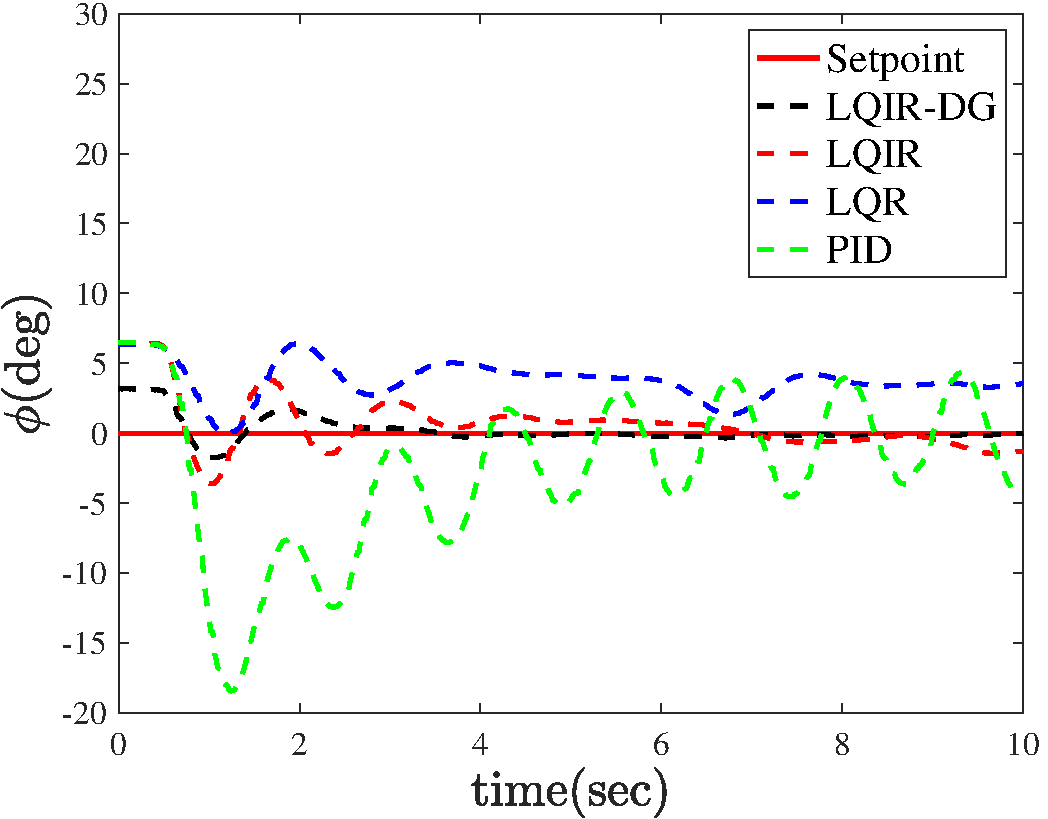
\includegraphics[width=.49\linewidth]{../Figure/implementation/lqidgvslqr/roll}}\subfloat[\label{fig:all_pitch}]{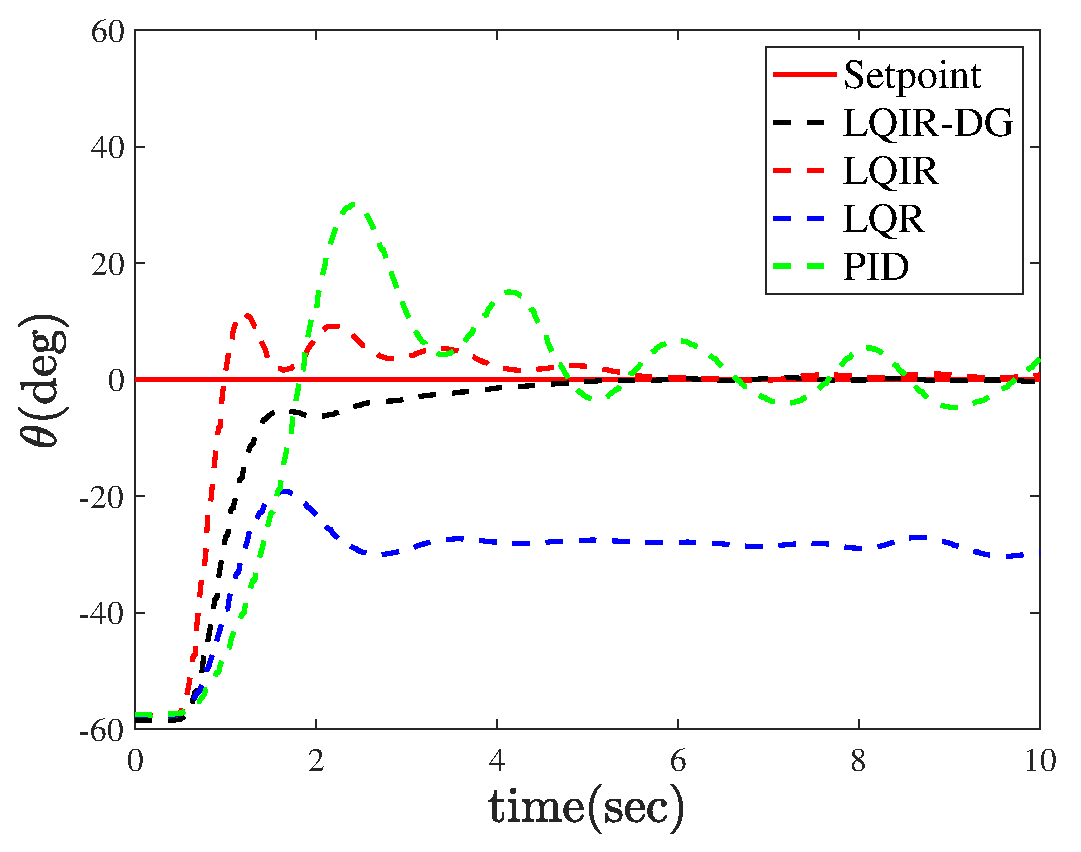
\includegraphics[width=.49\linewidth]{../Figure/implementation/lqidgvslqr/pitch}
	}
	\caption{The implementation results of the LQIR-DG Control Strategy with added weight on the roll and pitch axes in the three-degree-of-freedom coupling mode. \ref{sub@fig:all_roll} Comparison of the desired roll angle with the actual roll angle, \ref{sub@fig:all_pitch} Comparison of the desired pitch angle with the actual pitch angle.}
	\label{fig:compare}
\end{figure}

\begin{figure}[H]
	\centering
	{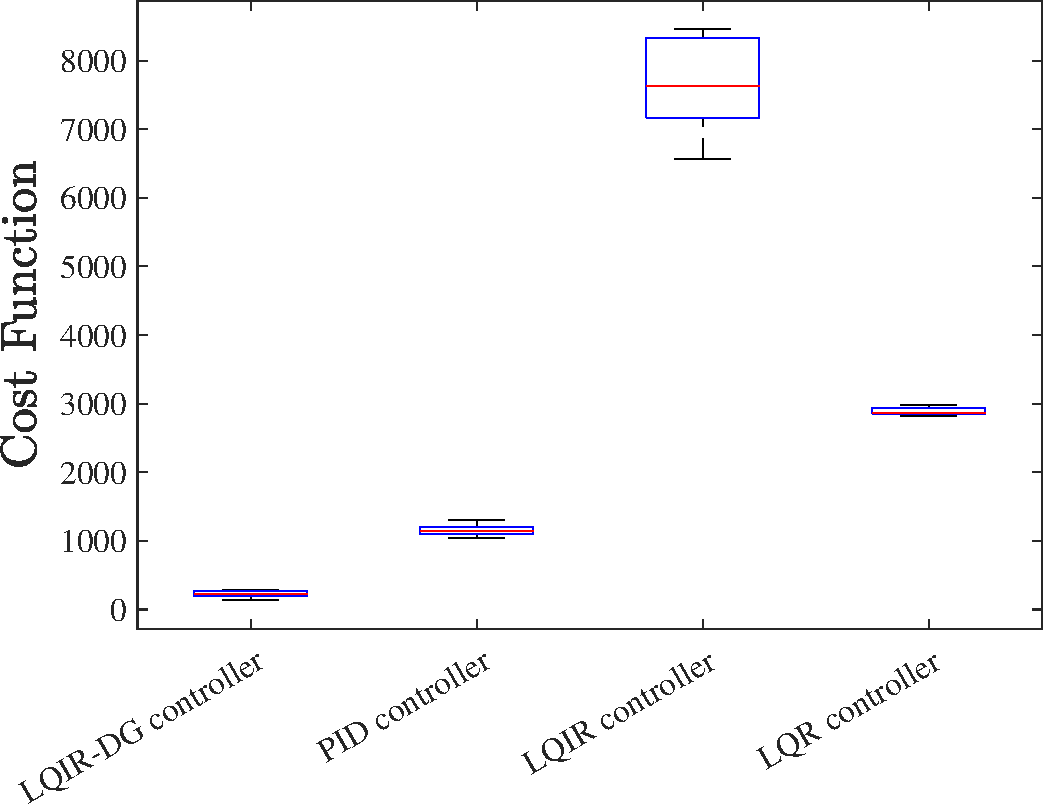
\includegraphics[width=.49\linewidth]{../Figure/implementation/box_plot/lqidgvsboxplot}
	}
	\caption{Comparative Analysis of the LQIR-DG Control Strategy versus LQR, LQIR, and PID Controllers using Quadratic Cost Function}
	\label{fig:compare_boxplot}
\end{figure}
\section{Conclusion}\label{sec:conclusion}
%% The Appendices part is started with the command \appendix;
%% appendix sections are then done as normal sections
%% \appendix

%% \section{}
%% \label{}

%% If you have bibdatabase file and want bibtex to generate the
%% bibitems, please use
%%
 \bibliographystyle{elsarticle-harv} 
 \bibliography{refs}

%% else use the following coding to input the bibitems directly in the
%% TeX file.

% \begin{thebibliography}{00}

%% \bibitem[Author(year)]{label}
%% Text of bibliographic item

% \bibitem[ ()]{}

% \end{thebibliography}
\end{document}

\endinput
%%
%% End of file `elsarticle-template-harv.tex'.
